%% This is file `elsarticle-template-1-num.tex',
%%
%% Copyright 2009 Elsevier Ltd
%%
%% This file is part of the 'Elsarticle Bundle'.
%% ---------------------------------------------
%%
%% It may be distributed under the conditions of the LaTeX Project Public
%% License, either version 1.2 of this license or (at your option) any
%% later version.  The latest version of this license is in
%%    http://www.latex-project.org/lppl.txt
%% and version 1.2 or later is part of all distributions of LaTeX
%% version 1999/12/01 or later.
%%
%% Template article for Elsevier's document class `elsarticle'
%% with numbered style bibliographic references
%%
%% $Id: elsarticle-template-1-num.tex 149 2009-10-08 05:01:15Z rishi $
%% $URL: http://lenova.river-valley.com/svn/elsbst/trunk/elsarticle-template-1-num.tex $
%%
\documentclass[preprint,12pt]{elsarticle}

%% Use the option review to obtain double line spacing
%% \documentclass[preprint,review,12pt]{elsarticle}

%% Use the options 1p,twocolumn; 3p; 3p,twocolumn; 5p; or 5p,twocolumn
%% for a journal layout:
%% \documentclass[final,1p,times]{elsarticle}
%% \documentclass[final,1p,times,twocolumn]{elsarticle}
%% \documentclass[final,3p,times]{elsarticle}
%% \documentclass[final,3p,times,twocolumn]{elsarticle}
%% \documentclass[final,5p,times]{elsarticle}
%% \documentclass[final,5p,times,twocolumn]{elsarticle}

%% The graphicx package provides the includegraphics command.
\usepackage{graphicx}
\usepackage{leftidx}
\usepackage{amsmath}

\usepackage[noend]{algpseudocode}

\usepackage{multirow}
\usepackage{algorithm}
\usepackage{algpseudocode}

\usepackage[top=2cm, bottom=2cm, left=2cm, right=2cm]{geometry}
\usepackage{algorithmicx}


%% The amssymb package provides various useful mathematical symbols
\usepackage{amssymb}
%% The amsthm package provides extended theorem environments
%% \usepackage{amsthm}

%% The lineno packages adds line numbers. Start line numbering with
%% \begin{linenumbers}, end it with \end{linenumbers}. Or switch it on
%% for the whole article with \linenumbers after \end{frontmatter}.
\usepackage{lineno}

%% natbib.sty is loaded by default. However, natbib options can be
%% provided with \biboptions{...} command. Following options are
%% valid:

%%   round  -  round parentheses are used (default)
%%   square -  square brackets are used   [option]
%%   curly  -  curly braces are used      {option}
%%   angle  -  angle brackets are used    <option>
%%   semicolon  -  multiple citations separated by semi-colon
%%   colon  - same as semicolon, an earlier confusion
%%   comma  -  separated by comma
%%   numbers-  selects numerical citations
%%   super  -  numerical citations as superscripts
%%   sort   -  sorts multiple citations according to order in ref. list
%%   sort&compress   -  like sort, but also compresses numerical citations
%%   compress - compresses without sorting
%%
%% \biboptions{comma,round}

% \biboptions{}

\journal{Journal Name}

\begin{document}

\begin{frontmatter}

%% Title, authors and addresses

\title{Scheduling Divisible Workloads from Multiple Sources in Regular and Torus Mesh}

%% use the tnoteref command within \title for footnotes;
%% use the tnotetext command for the associated footnote;
%% use the fnref command within \author or \address for footnotes;
%% use the fntext command for the associated footnote;
%% use the corref command within \author for corresponding author footnotes;
%% use the cortext command for the associated footnote;
%% use the ead command for the email address,
%% and the form \ead[url] for the home page:
%%
%% \title{Title\tnoteref{label1}}
%% \tnotetext[label1]{}
%% \author{Name\corref{cor1}\fnref{label2}}
%% \ead{email address}
%% \ead[url]{home page}
%% \fntext[label2]{}
%% \cortext[cor1]{}
%% \address{Address\fnref{label3}}
%% \fntext[label3]{}


%% use optional labels to link authors explicitly to addresses:
%% \author[label1,label2]{<author name>}
%% \address[label1]{<address>}
%% \address[label2]{<address>}

\author{Junwei Zhang}

\address{Stony Brook, New York}

\begin{abstract}
%% Text of abstract
This report is about multiple sources\cite{jia2010scheduling} workloads scheduling\cite{robertazzi1993processor} in regular mesh and torus mesh.
\end{abstract}

\begin{keyword}
Divisible Load Theory \sep Processor Equivalence \sep Voronoi Diagram \sep Optimal Mass Transport \sep Monte Carlo Method
\sep Manhattan Distance 
%% keywords here, in the form: keyword \sep keyword

%% MSC codes here, in the form: \MSC code \sep code
%% or \MSC[2008] code \sep code (2000 is the default)

\end{keyword}

\end{frontmatter}

%%
%% Start line numbering here if you want
%%
%%\linenumbers

%% main text
\subsection{Related Literature}

\subsubsection{Divisible Load Theory}
Crucial to our success in the single and multiple injection point cases, is the use of divisible load scheduling theory [refs].  Developed over the past few decades, it assumes load is a continuous variable that can be arbitrarily partitioned among processors and links in a network.  Use is made of the divisible load scheduling’s optimality principle [ref], which say makespan is minimized when one forces all processors to stop at the same time (intuitively otherwise one could transfer load from busy to idle processors to achieve a better solution).  This leads to a series of chained linear flow and processing equations that can be solved by linear equation techniques, often yielding recursive and even closed form solutions for quantities such as makespan and speedup. 

\subsubsection{Voronoi Diagrams}
In the context of multiple injection point models, this paper represents 
Jia  \cite{jia2010scheduling} proposes a genetic algorithm, which utilize a novel Graph Partitioning (GP) scheme to partition the network such that each source in the network gains a portion of network resources and then these sources cooperate to process their loads.  We utilize the Voronoi diagrams \cite{jia2010scheduling} in conjunction with divisible load scheduling for a significant applied problem. 

In mathematics, a Voronoi diagram \cite{fortune1995voronoi} a partitioning of a plane into regions based on distance to points in a specific subset of the plane. For each seed there is a corresponding region consisting of all points closer to that seed than to any other. These regions are called Voronoi cells. 

\subsection{Problem Description}
Networks on chips (NOC) represent the smallest networks that have been implemented to date \cite{robertazzi2017computer}.  A popular choice for the interconnection network on such networks on chips is the rectangular mesh.  It is straightforward to implement and is a natural choice for a planar chip layout.

Data to be processed can be inserted into the chip at one or more so-called “injection points”, that is node(s) in the mesh that forward the data to other nodes.  Beyond NOCs, injecting data into a parallel processor’s interconnection network has been done for some time, notably in IBM’s Bluegene machines \cite{krevat2002job}.  In this paper it is sought to determine, for a given set of injection points how, optimally or near-optimally, to assign load to different processors in a known timed pattern so as to process a load of data in a minimal amount of time (i.e. minimize makespan).  In this paper we succeed in presenting an optimal technique for single injection points in homogeneous meshes that involves no more complexity than linear equation solution.  For multiple injection points we present algorithms that produce near optimal solutions using Voronoi diagrams \cite{fortune1987sweepline} \cite{jia2010scheduling}.  The methodology presented here can be applied to a variety of switching/scheduling protocols besides those directly covered in this paper. 

In this paper, we investigate the virtual cut-through switching \cite{kermani1979virtual}.  In the virtual cut-through environment, a node can begin relaying the first part of a message (packet) along a transmission path as soon as it starts to arrive at the node , that is, it doesn't have to wait to receive the entire message before it can begin forwarding the message.

Equivalence computation \cite{robertazzi1993processor} is a technique, which consists of combining a cluster of processors as one whole equivalent processor to process a unit $1$ workload.

\section{Processor Equivalence}
In this section, we will discuss the power equivalence problem.
\\
I will present the closed-form equal formula about the load from three different kind of injection position,load from corner,boundary and inner grid position in regular mesh.
\\
In addition, considering the unit core with or without the front-end processor,the data transportation schema can be considered as two situation with front-end  and without front-end transportation.

\vspace*{5pt}

For a homogeneous regular mesh, which can be collapsed into an equivalent node, the notation is presented as follows.\\

\begin{itemize}

\item $\alpha_{0}$: The load fraction assigned to the root processor.
\item $\alpha_{i}$: The load fraction assigned to the $i$th processor.
\item $\omega_{i}$: The inverse computing speed on the $i$th processor.
\item $\omega_{eq}$: The inverse computing speed on an equivalent node collapsed from a regular mesh.
\item $z_{i}$: The inverse link speed on the $i$th link.
\item $T_{cp}$: Computing intensity constant.The entire load can be transmitted in $z_{i}T_{cp}$ on the $i$th processor.
\item $T_{cm}$: Communication intensity constant.The entire load can be transmitted in $z_{i}T_{cm}$ seconds over the $i$th link.
\item $T_{f,m}$: The finish time of the whole regular network.Here $T_{f,m}$ is equal to $\omega_{eq}T_{cp}$.
\item $T_{f,0}$: The finish time for the entire divisible load solved on the root processor.Here $T_{f,0}$ is equal to $1 \times \omega_{0}T_{cp}$, that is $\omega_{0}T_{cp}$.

\end{itemize}
\vspace*{5pt}
\subsection{With Front-end Schema}
\vspace*{5pt}
I investigate the simple case first and then deduce the more general closed form formula for the homogeneous regular mesh situation.
\vspace*{5pt}

\subsubsection{Load From Corner}
\begin{itemize}
\vspace*{5pt}
\item 2*2 regular mesh Fig.\ref{22f}
\item 2*3 regular mesh Fig.\ref{23f}
\item 2*n regular mesh,for example $n = 10$ Fig.\ref{210f}
\item 3*n regular mesh,for example $n = 8$ Fig.\ref{38f}
\item m*n regular mesh,for example $m = 5, n = 5$ Fig.\ref{410f}
\end{itemize}

According to Fig.\ref{22f},data injection position comes from corner.

There are four unit cores to handle the whole workload in the regular mesh.

\begin{figure}[h]
\centering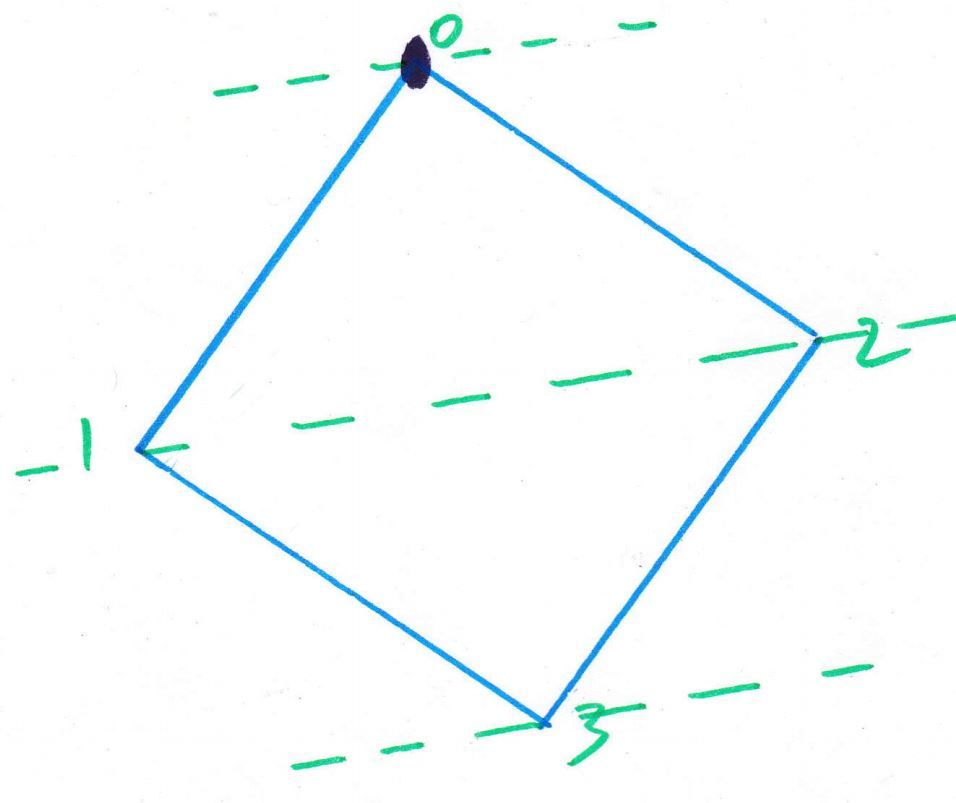
\includegraphics[width = 0.7\linewidth]{figure/c22_f}
\caption{2*2 regular mesh}
\label{22f}
\end{figure}


$$\alpha_{0} \omega T_{cp} = T_{f,m}$$ 
$$\alpha_{1} \omega T_{cp} = T_{f,m}$$
$$\alpha_{2} \omega T_{cp} = T_{f,m}$$
$$\alpha_{1}zT_{cm} + \alpha_{3}\omega T_{cp} = T_{f,m}$$
$$\sigma = \frac{zT_{cm}}{\omega T_{cp}}$$


\begin{equation}
{
\left[ \begin{array}{ccc}
1 & 2 & 1\\
1 & -1 & 0\\
0 & \sigma-1 & 1
\end{array} 
\right ]} \times \left[ \begin{array}{c}
\alpha_{0} \\
\alpha_{1} \\
\alpha_{3} 
\end{array} 
\right ] = \left[ \begin{array}{c}
1 \\
0 \\
0 
\end{array} 
\right ]
\end{equation}

\vspace*{50pt}
According to Fig.\ref{23f}, the data load injection comes from corner and there are
six cores to handle the whole workload.

\begin{figure}[h]
\centering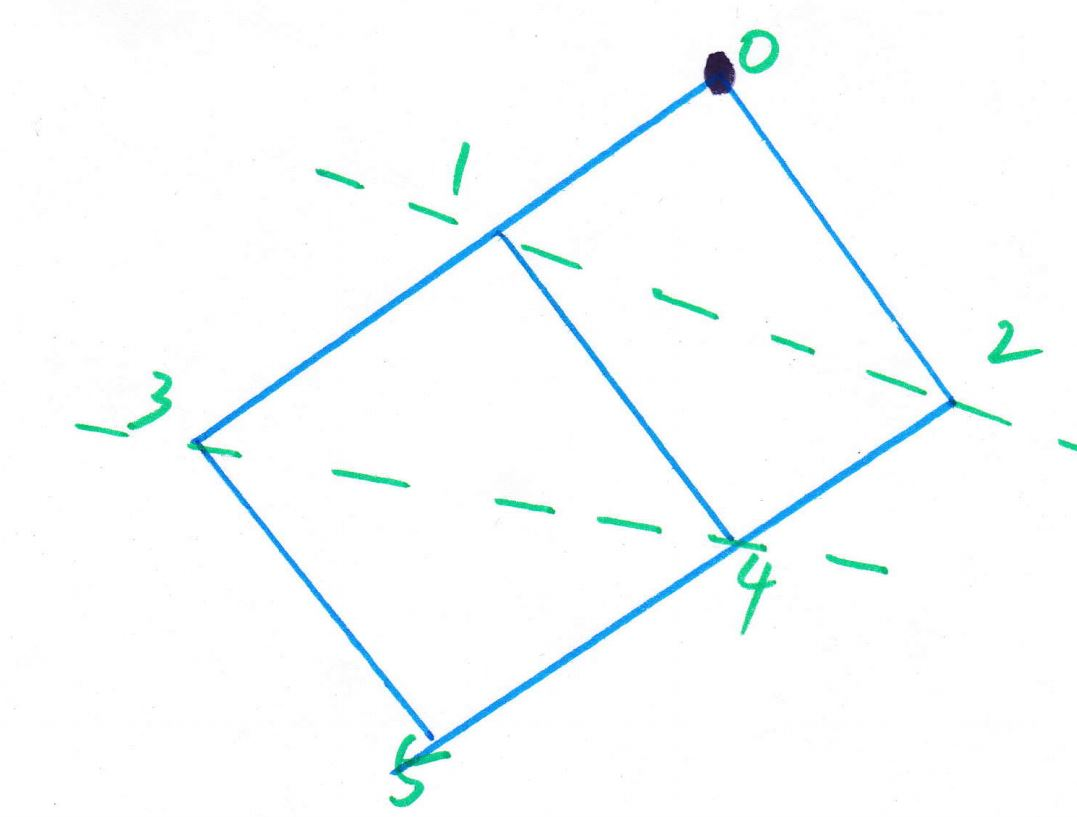
\includegraphics[width=0.7\linewidth]{figure/c23_f}
\caption{2*3 regular mesh}
\label{23f}
\end{figure}

$$\alpha_{0} \omega T_{cp} = T_{f,m}$$ 
$$\alpha_{1} \omega T_{cp} = T_{f,m}$$
$$\alpha_{2} \omega T_{cp} = T_{f,m}$$
$$\alpha_{1}zT_{cm} + \alpha_{3}\omega T_{cp} = T_{f,m}$$
$$\alpha_{2}zT_{cm} + \alpha_{4}\omega T_{cp} = T_{f,m}$$
$$(\alpha_{1} + \alpha_{3})zT_{cm} + \alpha_{5}\omega T_{cp} = T_{f,m}$$

$$\sigma = \frac{zT_{cm}}{\omega T_{cp}}$$
\begin{equation}
{
\left[ \begin{array}{cccc}
1 & 2 & 2 & 1\\
1 & -1 & 0 & 0\\
0 & \sigma-1 & 1 & 0\\
0 & \sigma-1 & \sigma & 1
\end{array} 
\right ]} \times \left[ \begin{array}{c}
\alpha_{0} \\
\alpha_{1} \\
\alpha_{3} \\
\alpha_{5}
\end{array} 
\right ] = \left[ \begin{array}{c}
1 \\
0 \\
0 \\
0
\end{array} 
\right ]
\end{equation}

\vspace*{50pt}

Considering the $2*n$ situation, the formula is:


$$\alpha_{0} \omega T_{cp} = T_{f,m}$$ 
$$\alpha_{1} \omega T_{cp} = T_{f,m}$$
$$\alpha_{2} \omega T_{cp} = T_{f,m}$$
$$\alpha_{1}zT_{cm} + \alpha_{3}\omega T_{cp} = T_{f,m}$$
$$\alpha_{2}zT_{cm} + \alpha_{4}\omega T_{cp} = T_{f,m}$$
$$(\alpha_{1} + \alpha_{3})zT_{cm} + \alpha_{5}\omega T_{cp} = T_{f,m}$$
$$\vdots$$
$$(\alpha_{1} + \alpha_{3} +\cdots + \alpha_{2 \times n - 1})zT_{cm} +\alpha_{2 \times n + 1} \omega T_{cp} = T_{f,m}$$
$$\sigma = \frac{zT_{cm}}{\omega T_{cp}}$$

\vspace*{50pt}
For example, the $n = 10$ Fig. \ref{210f}, the formula as follows:

\begin{figure}[h]
\centering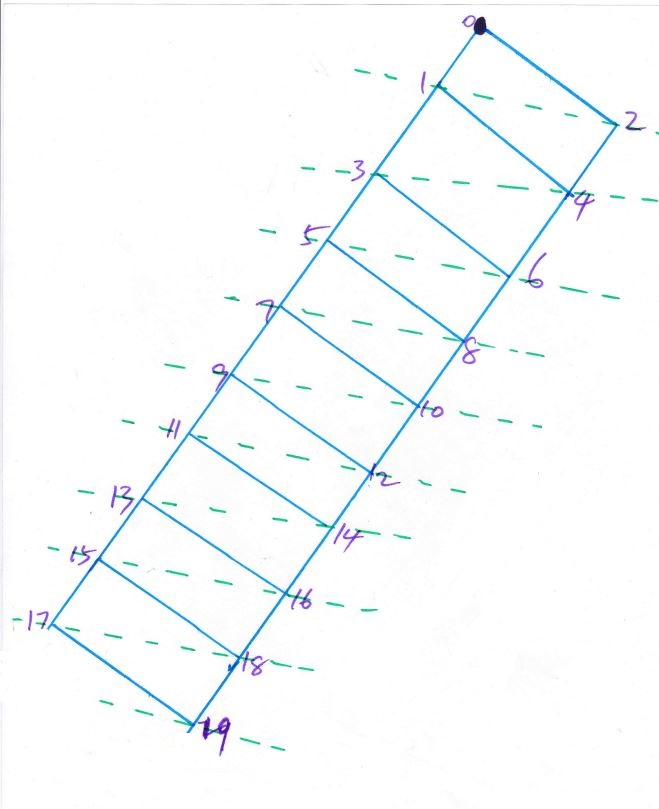
\includegraphics[width=0.7\linewidth]{figure/c210_f}
\caption{2*n $(n = 10)$ regular mesh}
\label{210f}
\end{figure}


\begin{equation}
{
\left[ \begin{array}{ccccccc}
1 & 2 & 2 & \cdots & 2 & 2 & 1\\
1 & -1 & 0 & \cdots& 0 & 0 & 0\\
0 & \sigma-1 & 1 & \cdots & 0 & 0 & 0 \\
0 & \sigma-1 & \sigma & 1 & 0 & \cdots & 0 \\
0 & \sigma-1 & \sigma & \sigma & 1 & 0 & 0 \\
\vdots & \vdots & \vdots  &   \vdots & \ddots & \ddots\\
0 & \sigma-1 & \sigma & \cdots & \sigma & \sigma & 1
\end{array} 
\right ]} \times \left[ \begin{array}{c}
\alpha_{0} \\
\alpha_{1} \\
\alpha_{3} \\
\alpha_{5} \\
\vdots \\
\alpha_{2 \times n - 1}\\
\alpha_{2 \times n + 1}
\end{array} 
\right ] = \left[ \begin{array}{c}
1 \\
0 \\
0 \\
0 \\
\vdots \\
0
\end{array} 
\right ]
\end{equation}

So the Speedup is $$\frac{1}{\alpha_{0}}$$.
\vspace*{50pt}


\vspace*{80pt}
Consider more general case Fig. \ref{38f}.

\begin{figure}[h]
\centering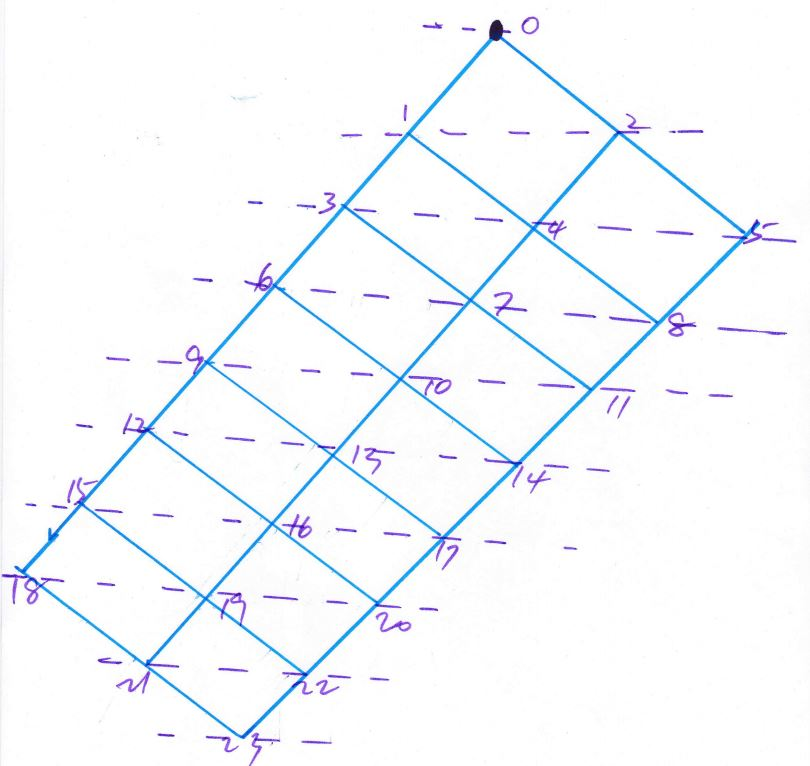
\includegraphics[width=0.7\linewidth]{figure/c38_f}
\caption{3*n $n = 8$ regular mesh}
\label{38f}
\end{figure}

The closed formula groups are presented as following:

\begin{equation}
{
\left[ \begin{array}{cccccccccc}
1 & 2 & 3 & 3 & 3 & 3 & 3 & 3 & 2 & 1\\
1 & -1 & 0 & 0 & 0 & 0 & 0 & 0 & 0 & 0\\
0 & \sigma-1 & 1 & 0 & 0 & 0 & 0 & 0 & 0 & 0 \\
0 & \sigma-1 & \sigma & 1 & 0 & 0 & 0 & 0 & 0 & 0 \\
0 & \sigma-1 & \sigma & \sigma & 1 & 0 & 0 & 0 & 0 & 0\\
0 & \sigma-1 & \sigma & \sigma & \sigma & 1 & 0 & 0 & 0 & 0\\
0 & \sigma-1 & \sigma & \sigma & \sigma & \sigma & 1 & 0 & 0 & 0\\
0 & \sigma-1 & \sigma & \sigma & \sigma & \sigma & \sigma & 1 & 0 & 0\\
0 & \sigma-1 & \sigma & \sigma & \sigma & \sigma & \sigma & \sigma & 1 & 0\\
0 & \sigma-1 & \sigma & \sigma & \sigma & \sigma & \sigma & \sigma & \sigma & 1 \\
\end{array} 
\right ]} \times \left[ \begin{array}{c}
\alpha_{0} \\
\alpha_{1} \\
\alpha_{3} \\
\alpha_{6} \\
\alpha_{9} \\
\alpha_{12}\\
\alpha_{15}\\
\alpha_{18}\\
\alpha_{21}\\
\alpha_{23}
\end{array} 
\right ] = \left[ \begin{array}{c}
1 \\
0 \\
0 \\
0 \\
\vdots \\
0
\end{array} 
\right ]
\end{equation}


\vspace*{50pt}
Consider more general case Fig.\ref{410f} the closed formula groups are presented as following:

\begin{figure}[h]
\centering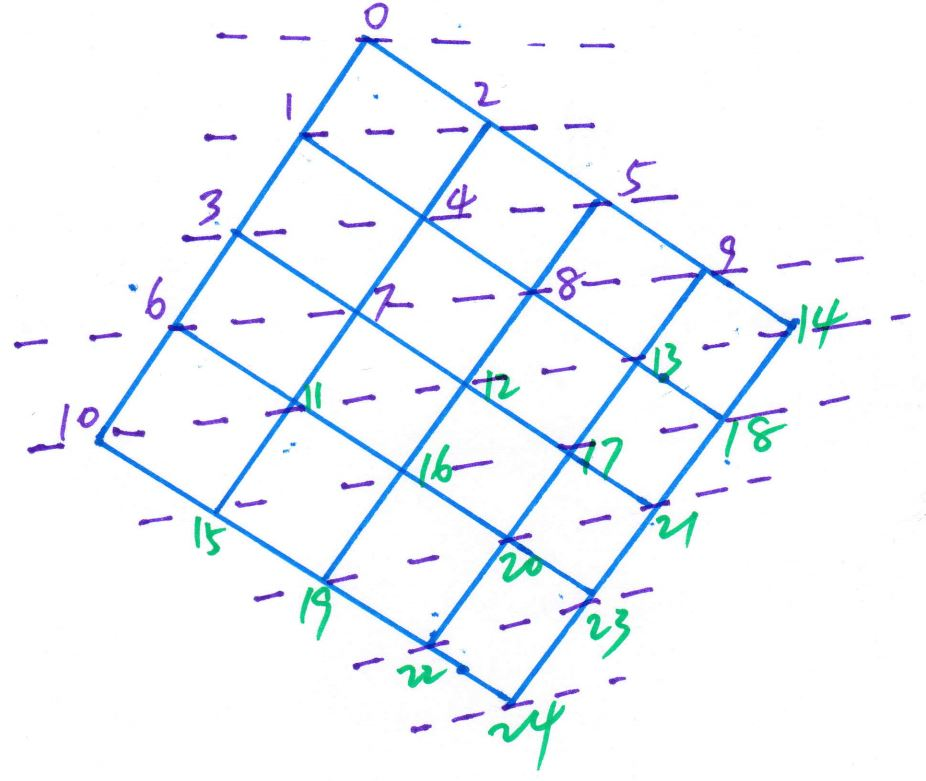
\includegraphics[width=0.7\linewidth]{figure/c410_f}
\caption{m*n $m = 5$, $n = 5$ regular mesh}
\label{410f}
\end{figure}


\begin{equation}
{
\left[ \begin{array}{ccccccccc}
1 & 2 & 3 & 4 & 5 & 4 & 3 & 2 & 1\\
1 & -1 & 0 & 0 & 0 & 0 & 0 & 0& 0\\
0 & \sigma-1 & 1 & 0 & 0 & 0 &0 & 0 & 0 \\
0 & \sigma-1 & \sigma & 1 & 0 & 0 & 0 & 0 & 0 \\
0 & \sigma-1 & \sigma & \sigma & 1 & 0 & 0 & 0 & 0\\
0 & \sigma-1 & \sigma & \sigma & \sigma & 1 & 0& 0 & 0\\
0 & \sigma-1 & \sigma & \sigma & \sigma & \sigma & 1 & 0 & 0\\
0 & \sigma-1 & \sigma & \sigma & \sigma & \sigma & \sigma & 1 & 0\\
0 & \sigma-1 & \sigma & \sigma & \sigma & \sigma & \sigma & \sigma & 1\\
\end{array} 
\right ]} \times \left[ \begin{array}{c}
\alpha_{0} \\
\alpha_{1} \\
\alpha_{3} \\
\alpha_{6} \\
\alpha_{10} \\
\alpha_{15}\\
\alpha_{19}\\
\alpha_{22}\\
\alpha_{24}
\end{array} 
\right ] = \left[ \begin{array}{c}
1 \\
0 \\
0 \\
0 \\
\vdots \\
0
\end{array} 
\right ]
\end{equation}

\vspace*{50pt}

\subsubsection{Load From Boundary Grid Position}
The data injection position lays on the boundary Fig.\ref{e33f} and the regular mesh is 3*3 situation.

\begin{figure}[h]
\centering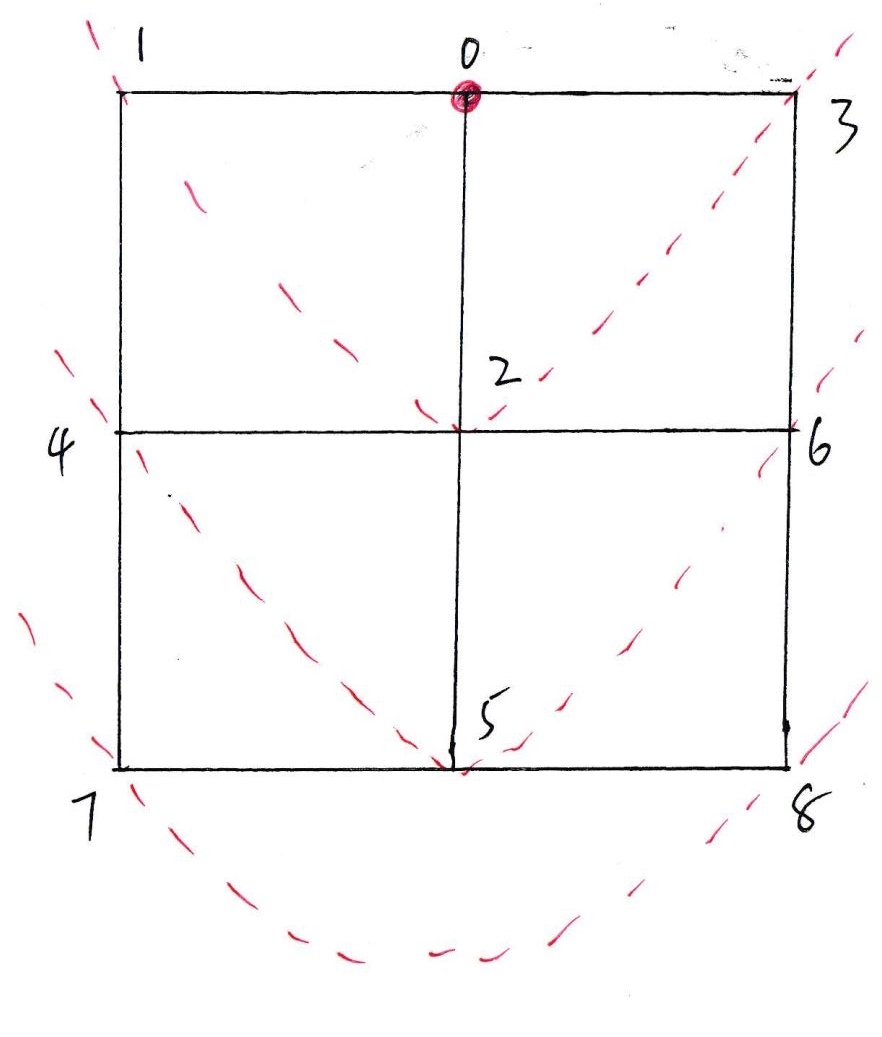
\includegraphics[width= 0.7 \linewidth]{figure/e33_f}
\caption{Data injection position on the boundary of 3*3 regular mesh}
\label{e33f}
\end{figure}

The equation for the boundary data injection condition as follows:

$$\alpha_{0} \omega T_{cp} = T_{f,m}$$ 
$$\alpha_{1} \omega T_{cp} = T_{f,m}$$
$$\alpha_{2} \omega T_{cp} = T_{f,m}$$
$$\alpha_{3} \omega T_{cp} = T_{f,m}$$
$$\alpha_{1}zT_{cm} + \alpha_{4}\omega T_{cp} = T_{f,m}$$
$$\alpha_{2}zT_{cm} + \alpha_{5}\omega T_{cp} = T_{f,m}$$
$$\alpha_{3}zT_{cm} + \alpha_{6}\omega T_{cp} = T_{f,m}$$
$$(\alpha_{1} + \alpha_{4})zT_{cm} + \alpha_{7}\omega T_{cp} = T_{f,m}$$
$$(\alpha_{2} + \alpha_{5})zT_{cm} + \alpha_{8}\omega T_{cp} = T_{f,m}$$

$$\sigma = \frac{zT_{cm}}{\omega T_{cp}}$$

\vspace*{50pt}

\begin{equation}
{
\left[ \begin{array}{cccc}
1 & 3 & 3 & 2\\
1 & -1 & 0 & 0\\
0 & \sigma-1 & 1 & 0\\
0 & \sigma-1 & \sigma & 1
\end{array} 
\right ]} \times \left[ \begin{array}{c}
\alpha_{0} \\
\alpha_{1} \\
\alpha_{4} \\
\alpha_{7}
\end{array} 
\right ] = \left[ \begin{array}{c}
1 \\
0 \\
0 \\
0
\end{array} 
\right ]
\end{equation}

\vspace*{50pt}

\subsubsection{Load From Inner Grid}
\vspace*{5pt}
The data injection position lays on the inner grid position Fig.\ref{i33f} and the regular mesh is 3*3 situation.

\begin{figure}[h]
\centering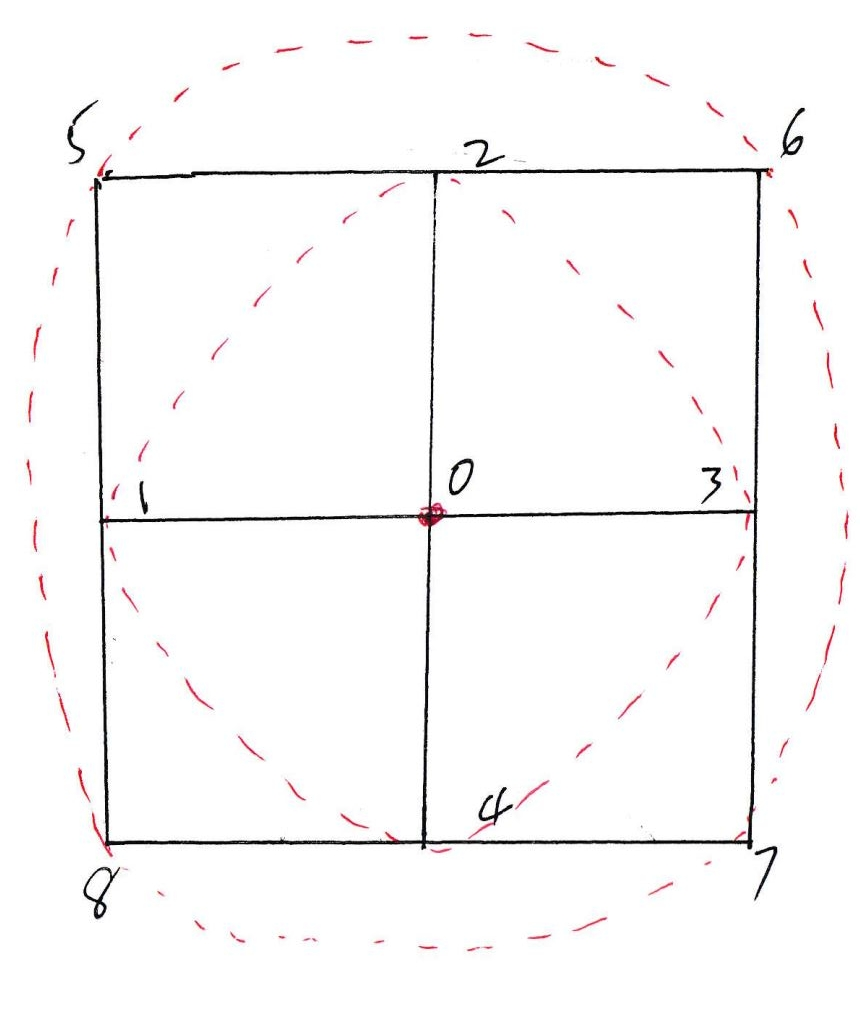
\includegraphics[width= 0.7\linewidth]{figure/i33_f}
\caption{Data injection position on the inner grid position of 3*3 regular mesh}
\label{i33f}
\end{figure}

$$\alpha_{0} \omega T_{cp} = T_{f,m}$$ 
$$\alpha_{1} \omega T_{cp} = T_{f,m}$$
$$\alpha_{2} \omega T_{cp} = T_{f,m}$$
$$\alpha_{3} \omega T_{cp} = T_{f,m}$$
$$\alpha_{4} \omega T_{cp} = T_{f,m}$$
$$\alpha_{1}zT_{cm} + \alpha_{5}\omega T_{cp} = T_{f,m}$$
$$\alpha_{1}zT_{cm} + \alpha_{6}\omega T_{cp} = T_{f,m}$$
$$\alpha_{1}zT_{cm} + \alpha_{7}\omega T_{cp} = T_{f,m}$$
$$\alpha_{1}zT_{cm} + \alpha_{8}\omega T_{cp} = T_{f,m}$$

The equation for the boundary condition as follows:

$$\sigma = \frac{zT_{cm}}{\omega T_{cp}}$$

\vspace*{20pt}

\begin{equation}
{
\left[ \begin{array}{ccc}
1 & 4 & 4 \\
1 & -1 & 0\\
0 & \sigma-1 & 1\\
\end{array} 
\right ]} \times \left[ \begin{array}{c}
\alpha_{0} \\
\alpha_{1} \\
\alpha_{5} \\
\end{array} 
\right ] = \left[ \begin{array}{c}
1 \\
0 \\
0 
\end{array} 
\right ]
\end{equation}


\subsection{General Case}
\begin{equation}
{
\left[ \begin{array}{ccccccc}
1 & m_{1} & m_{2} & \cdots & m_{n-2} & m_{n-1} & m_{n}\\
1 & -1 & 0 & \cdots& 0 & 0 & 0\\
0 & \sigma -1 & 1 & \cdots & 0 & 0 & 0 \\
0 & \sigma -1 & \sigma & 1 & 0 & \cdots & 0 \\
0 & \sigma -1 & \sigma & \sigma & 1 & 0 & 0 \\
\vdots & \vdots & \vdots  &   \vdots & \ddots & \ddots\\
0 & \sigma -1 & \sigma & \cdots & \sigma & \sigma & 1
\end{array} 
\right ]} \times \left[ \begin{array}{c}
\alpha_{l_{0}} \\
\alpha_{l_{1}} \\
\alpha_{l_{2}} \\
\alpha_{l_{3}} \\
\vdots \\
\alpha_{l_{n-1}}\\
\alpha_{l_{n}}
\end{array} 
\right ] = \left[ \begin{array}{c}
1 \\
0 \\
0 \\
0 \\
\vdots \\
0
\end{array} 
\right ]
\end{equation}











\vspace*{5pt}
\subsubsection{Workstation without front-end}

\vspace*{50pt}

We investigate the simple case first and then deduce the more general closed form formula for the regular mesh situation.

\subsection{Load From Corner}
\begin{itemize}

\item 2*2 regular mesh Fig.\ref{22f}
\item 2*3 regular mesh Fig.\ref{23f}
\item 2*n regular mesh,for example $n = 10$ Fig.\ref{210f}
\item 3*n regular mesh,for example $n = 8$ Fig.\ref{38f}
\item m*n regular mesh,for example $m = 5, n = 5$ Fig.\ref{410f}

\end{itemize}

According to Fig.\ref{22f},data injection position comes from corner unit processor.

There are four cores to handle the whole workload in the regular mesh.

$$\alpha_{0} \omega T_{cp} = T_{f,m}$$ 
$$\alpha_{1}zT_{cm} + \alpha_{1} \omega T_{cp} = T_{f,m}$$
$$\alpha_{2}zT_{cm} + \alpha_{2} \omega T_{cp} = T_{f,m}$$
$$(\alpha_{1} + \alpha_{3})zT_{cm} + \alpha_{3}\omega T_{cp} = T_{f,m}$$
$$\sigma = \frac{zT_{cm}}{\omega T_{cp}}$$

\begin{equation}
{
\left[ \begin{array}{ccc}
1 & 2 & 1\\
1 & -(\sigma + 1) & 0\\
1 & -\sigma & -(\sigma + 1)
\end{array} 
\right ]} \times \left[ \begin{array}{c}
\alpha_{0} \\
\alpha_{1} \\
\alpha_{3} 
\end{array} 
\right ] = \left[ \begin{array}{c}
1 \\
0 \\
0 
\end{array} 
\right ]
\end{equation}

\vspace*{50pt}

According to Fig.\ref{23f}, the formula groups are

$$\alpha_{0} \omega T_{cp} = T_{f,m}$$ 
$$\alpha_{1}zT_{cm} + \alpha_{1} \omega T_{cp} = T_{f,m}$$
$$\alpha_{2}zT_{cm} + \alpha_{2} \omega T_{cp} = T_{f,m}$$
$$(\alpha_{1} + \alpha_{3})zT_{cm} + \alpha_{3}\omega T_{cp} = T_{f,m}$$
$$(\alpha_{1} + \alpha_{4})zT_{cm} + \alpha_{4}\omega T_{cp} = T_{f,m}$$
$$(\alpha_{1} + \alpha_{3} + \alpha_{5})zT_{cm} + \alpha_{5}\omega T_{cp} = T_{f,m}$$

\begin{equation}
{
\left[ \begin{array}{cccc}
1 & 2 & 2 & 1\\
1 & -(\sigma + 1) & 0 & 0\\
1 & -\sigma & -(\sigma + 1) & 0\\
1 & -\sigma & -\sigma & -(\sigma + 1)
\end{array} 
\right ]} \times \left[ \begin{array}{c}
\alpha_{0} \\
\alpha_{1} \\
\alpha_{3} \\
\alpha_{5}
\end{array} 
\right ] = \left[ \begin{array}{c}
1 \\
0 \\
0 \\
0
\end{array} 
\right ]
\end{equation}

$$\sigma = \frac{zT_{cm}}{\omega T_{cp}}$$

the speedup ratio is:
$\frac{1}{\alpha_{0}}$

\vspace*{50pt}

According to the 2*n regular mesh, the formula equation group as follows:

$$\alpha_{1}zT_{cm} + \alpha_{1} \omega T_{cp} = T_{f,m}$$
$$\alpha_{2}zT_{cm} + \alpha_{2} \omega T_{cp} = T_{f,m}$$
$$(\alpha_{1} + \alpha_{3})zT_{cm} + \alpha_{3}\omega T_{cp} = T_{f,m}$$
$$(\alpha_{1} + \alpha_{4})zT_{cm} + \alpha_{4}\omega T_{cp} = T_{f,m}$$

$$(\alpha_{1} + \alpha_{3} + \alpha_{5})zT_{cm} + \alpha_{5}\omega T_{cp} = T_{f,m}$$
$$\vdots$$
$$(\alpha_{1} + \alpha_{3} +\cdots + \alpha_{2 \times n + 1})zT_{cm} +\alpha_{2 \times n + 1} \omega T_{cp} = T_{f,m}$$

$$\sigma = \frac{zT_{cm}}{\omega T_{cp}}$$

\begin{equation}
{
\left[ \begin{array}{ccccccc}
1 & 2 & 2 & \cdots & 2 & 2 & 1\\
1 & -(\sigma + 1) & 0 & \cdots& 0 & 0 & 0\\
1 & -\sigma & -(\sigma + 1) & \cdots & 0 & 0 & 0 \\
1 & -\sigma & -\sigma & -(\sigma + 1) & 0 & \cdots & 0 \\
1 & -\sigma & -\sigma & -\sigma & -(\sigma + 1) & 0 & 0 \\
\vdots & \vdots & \vdots  &   \vdots & \ddots & \ddots\\
1 & -\sigma & -\sigma & \cdots & -\sigma & -\sigma & -(\sigma + 1)
\end{array} 
\right ]} \times \left[ \begin{array}{c}
\alpha_{0} \\
\alpha_{1} \\
\alpha_{3} \\
\alpha_{5} \\
\vdots \\
\alpha_{2 \times n - 1}\\
\alpha_{2 \times n + 1}
\end{array} 
\right ] = \left[ \begin{array}{c}
1 \\
0 \\
0 \\
0 \\
\vdots \\
0
\end{array} 
\right ]
\end{equation}

So the Speedup is $$\frac{1}{\alpha_{0}}$$

\vspace*{50pt}

According to the Fig.\ref{38f}, the matrix is:
We use ${\sigma}^{\star}$ to present the $-(\sigma + 1)$

\begin{small}
\begin{equation}
{
\left[ \begin{array}{cccccccccc}
1 & 2 & 3 & 3 & 3 & 3 & 3 & 3 & 2 & 1\\
1 & {\sigma}^{\star} & 0 & 0 & 0 & 0 & 0 & 0 & 0 & 0\\
1 & -\sigma & {\sigma}^{\star} & 0 & 0 & 0 & 0 & 0 & 0 & 0 \\
1 & -\sigma & -\sigma & {\sigma}^{\star} & 0 & 0 & 0 & 0 & 0 & 0 \\
1 & -\sigma & -\sigma & -\sigma & {\sigma}^{\star} & 0 & 0 & 0 & 0 & 0\\
1 & -\sigma & -\sigma & -\sigma & -\sigma & {\sigma}^{\star} & 0 & 0 & 0 & 0\\
1 & -\sigma & -\sigma & -\sigma & -\sigma & -\sigma & {\sigma}^{\star} & 0 & 0 & 0\\
1 & -\sigma & -\sigma & -\sigma & -\sigma & -\sigma & -\sigma & {\sigma}^{\star} & 0 & 0\\
1 & -\sigma & -\sigma & -\sigma & -\sigma & -\sigma & -\sigma & -\sigma & {\sigma}^{\star} & 0\\
1 & -\sigma & -\sigma & -\sigma & -\sigma & -\sigma & -\sigma & -\sigma & -\sigma & -{\sigma}^{\star} \\
\end{array} 
\right ]} \times \left[ \begin{array}{c}
\alpha_{0} \\
\alpha_{1} \\
\alpha_{3} \\
\alpha_{6} \\
\alpha_{9} \\
\alpha_{12}\\
\alpha_{15}\\
\alpha_{18}\\
\alpha_{21}\\
\alpha_{23}
\end{array} 
\right ] = \left[ \begin{array}{c}
1 \\
0 \\
0 \\
0 \\
\vdots \\
0
\end{array} 
\right ]
\end{equation}
\end{small}


\vspace*{50pt}
According to the Fig. \ref{410f}, the formula groups as follows:
We use ${\sigma}^{\star}$ to present the $-(\sigma + 1)$

\begin{equation}
{
\left[ \begin{array}{ccccccccc}
1 & 2 & 3 & 4 & 5 & 4 & 3 & 2 & 1\\
1 & {\sigma}^{\star} & 0 & 0 & 0 & 0 & 0 & 0 & 0\\
1 & -\sigma & {\sigma}^{\star} & 0 & 0 & 0 & 0& 0 & 0 \\
1 & -\sigma & -\sigma & {\sigma}^{\star} & 0 &0 & 0 & 0 & 0 \\
1 & -\sigma & -\sigma & -\sigma & {\sigma}^{\star} & 0 & 0 & 0 & 0\\
1 & -\sigma & -\sigma & -\sigma & -\sigma & {\sigma}^{\star} & 0 & 0 & 0\\
1 & -\sigma & -\sigma & -\sigma & -\sigma & -\sigma & {\sigma}^{\star} & 0 & 0\\
1 & -\sigma & -\sigma & -\sigma & -\sigma & -\sigma & -\sigma & {\sigma}^{\star} &0\\
1 & -\sigma & -\sigma & -\sigma & -\sigma & -\sigma & -\sigma & -\sigma & {\sigma}^{\star}\\
\end{array} 
\right ]} \times \left[ \begin{array}{c}
\alpha_{0} \\
\alpha_{1} \\
\alpha_{3} \\
\alpha_{6} \\
\alpha_{10} \\
\alpha_{15}\\
\alpha_{19}\\
\alpha_{22}\\
\alpha_{24}
\end{array} 
\right ] = \left[ \begin{array}{c}
1 \\
0 \\
0 \\
0 \\
\vdots \\
0
\end{array} 
\right ]
\end{equation}


\vspace*{50pt}
\subsubsection{Load From Boundary Grid Position}
The data injection position lays on the boundary Fig.\ref{e33f} and the regular mesh is 3*3 situation.

$$\alpha_{0} \omega T_{cp} = T_{f,m}$$ 
$$\alpha_{1}zT_{cm} + \alpha_{1} \omega T_{cp} = T_{f,m}$$
$$\alpha_{2}zT_{cm} + \alpha_{2} \omega T_{cp} = T_{f,m}$$
$$\alpha_{3}zT_{cm} + \alpha_{3} \omega T_{cp} = T_{f,m}$$
$$(\alpha_{1} + \alpha_{4})zT_{cm} + \alpha_{4}\omega T_{cp} = T_{f,m}$$
$$(\alpha_{2} + \alpha_{5})zT_{cm} + \alpha_{5}\omega T_{cp} = T_{f,m}$$
$$(\alpha_{3} + \alpha_{6})zT_{cm} + \alpha_{6}\omega T_{cp} = T_{f,m}$$
$$(\alpha_{1} + \alpha_{4} +\alpha_{7})zT_{cm} + \alpha_{7}\omega T_{cp} = T_{f,m}$$
$$(\alpha_{1} + \alpha_{4} +\alpha_{8})zT_{cm} + \alpha_{8}\omega T_{cp} = T_{f,m}$$

The equation for the boundary condition as follows:

$$\sigma = \frac{zT_{cm}}{\omega T_{cp}}$$
\begin{equation}
{
\left[ \begin{array}{cccc}
1 & 3 & 3 & 2\\
1 & -(\sigma + 1) & 0 & 0\\
1 & -\sigma & -(\sigma + 1) & 0\\
1 & -\sigma & -\sigma & -(\sigma + 1)
\end{array} 
\right ]} \times \left[ \begin{array}{c}
\alpha_{0} \\
\alpha_{1} \\
\alpha_{4} \\
\alpha_{7}
\end{array} 
\right ] = \left[ \begin{array}{c}
1 \\
0 \\
0 \\
0
\end{array} 
\right ]
\end{equation}



\vspace*{50pt}
\subsubsection{Load From Inner Grid}
The data injection position lays on the inner grid position Fig.\ref{i33f} and the regular mesh is 3*3 situation.

$$\alpha_{0} \omega T_{cp} = T_{f,m}$$ 
$$\alpha_{1}zT_{cm} + \alpha_{1} \omega T_{cp} = T_{f,m}$$
$$\alpha_{2}zT_{cm} + \alpha_{2} \omega T_{cp} = T_{f,m}$$
$$\alpha_{3}zT_{cm} + \alpha_{3} \omega T_{cp} = T_{f,m}$$
$$\alpha_{4}zT_{cm} + \alpha_{4} \omega T_{cp} = T_{f,m}$$
$$(\alpha_{1} + \alpha_{5})zT_{cm} + \alpha_{5}\omega T_{cp} = T_{f,m}$$
$$(\alpha_{2} + \alpha_{6})zT_{cm} + \alpha_{6}\omega T_{cp} = T_{f,m}$$
$$(\alpha_{3} + \alpha_{7})zT_{cm} + \alpha_{7}\omega T_{cp} = T_{f,m}$$
$$(\alpha_{4} + \alpha_{8})zT_{cm} + \alpha_{8}\omega T_{cp} = T_{f,m}$$

The equation for the boundary data injection condition as follows:

$$\sigma = \frac{zT_{cm}}{\omega T_{cp}}$$

\begin{equation}
{
\left[ \begin{array}{ccc}
1 & 4 & 4 \\
1 & -(\sigma + 1) & 0\\
1 & -\sigma & -(\sigma + 1)\\
\end{array} 
\right ]} \times \left[ \begin{array}{c}
\alpha_{0} \\
\alpha_{1} \\
\alpha_{5} \\
\end{array} 
\right ] = \left[ \begin{array}{c}
1 \\
0 \\
0 
\end{array} 
\right ]
\end{equation}
\vspace*{50pt}


\subsubsection{General Case}
\begin{equation}
{
\left[ \begin{array}{ccccccc}
1 & m_{1} & m_{2} & \cdots & m_{n-2} & m_{n-1} & m_{n}\\
1 & -(\sigma + 1) & 0 & \cdots& 0 & 0 & 0\\
1 & -\sigma & -(\sigma + 1) & \cdots & 0 & 0 & 0 \\
1 & -\sigma & -\sigma & -(\sigma + 1) & 0 & \cdots & 0 \\
1 & -\sigma & -\sigma & -\sigma & -(\sigma + 1) & 0 & 0 \\
\vdots & \vdots & \vdots  &   \vdots & \ddots & \ddots\\
1 & -\sigma & -\sigma & \cdots & -\sigma & -\sigma & -(\sigma + 1)
\end{array} 
\right ]} \times \left[ \begin{array}{c}
\alpha_{l_{0}} \\
\alpha_{l_{1}} \\
\alpha_{l_{2}} \\
\alpha_{l_{3}} \\
\vdots \\
\alpha_{l_{n-1}}\\
\alpha_{l_{n}}
\end{array} 
\right ] = \left[ \begin{array}{c}
1 \\
0 \\
0 \\
0 \\
\vdots \\
0
\end{array} 
\right ]
\end{equation}
\vspace*{5pt}
\subsubsection{Speedup Result between front-end schema and without front-end schema}
\begin{figure}[h]
\centering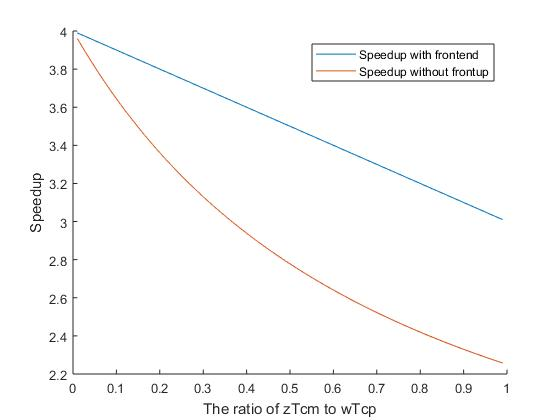
\includegraphics[width=0.7\linewidth]{figure/c22}
\caption{Speedup vs $\sigma$ value in 2*2 regular mesh}
\label{22}
\end{figure}

\begin{figure}[h]
\centering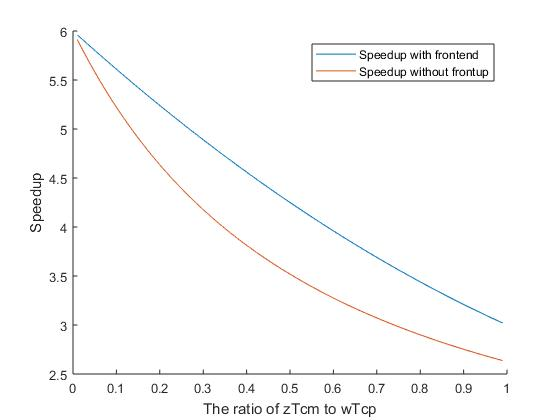
\includegraphics[width=0.7\linewidth]{figure/c23}
\caption{Speedup vs $\sigma$ value in 2*3 regular mesh}
\label{23}
\end{figure}

\begin{figure}[h]
\centering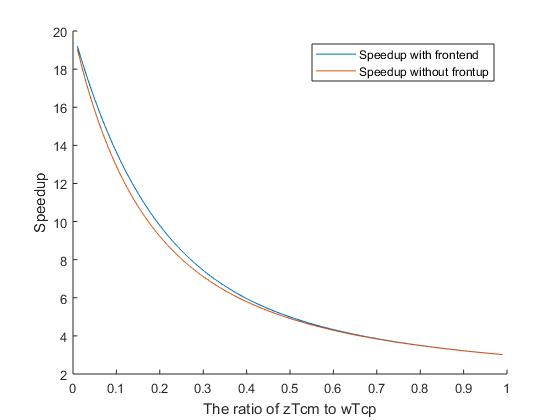
\includegraphics[width=0.7\linewidth]{figure/c210}
\caption{Speedup vs $\sigma$ value in 2*10 regular mesh}
\label{210}
\end{figure}

\begin{figure}[h]
\centering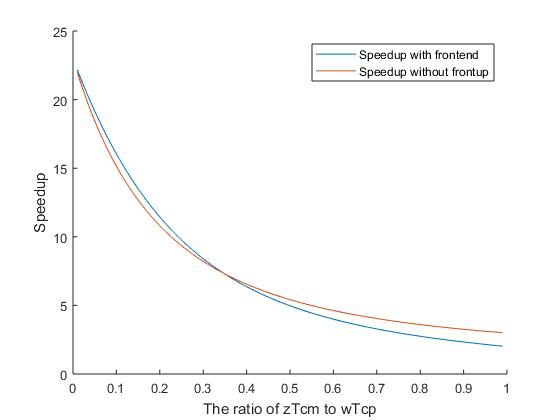
\includegraphics[width=0.7\linewidth]{figure/c38}
\caption{Speedup vs $\sigma$ value in 3*8 regular mesh}
\label{38}
\end{figure}

\begin{figure}[h]
\centering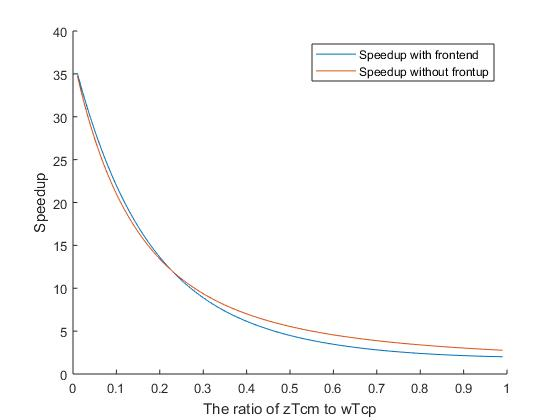
\includegraphics[width=0.7\linewidth]{figure/c410}
\caption{Speedup vs $\sigma$ value in 4*10 regular mesh}
\label{410}
\end{figure}






\section{Sensitivity Analysis}

\vspace*{50pt}
In this section, we investigate the sensitivity of regular mesh equal speedup analysis.

\vspace*{50pt}
\subsection{Front End Schema}

\subsubsection{2*n regular mesh}
Considering the $2*n $ regular mesh Fig .\ref{210f} and the data injection position on the corner.

The speedup vs the number of cores relationship Fig.\ref{corner2n} and Fig.\ref{corner2n2} as follows:

\vspace*{15pt}
\begin{itemize}
\item we can see as the number of cores grows and the equal computational grow as well. 
\item At the same, the $\sigma$ value plays an import role, especially $\sigma > 0.25$. The speedup drops dramatically.
\end{itemize}


\begin{figure}[h]
\centering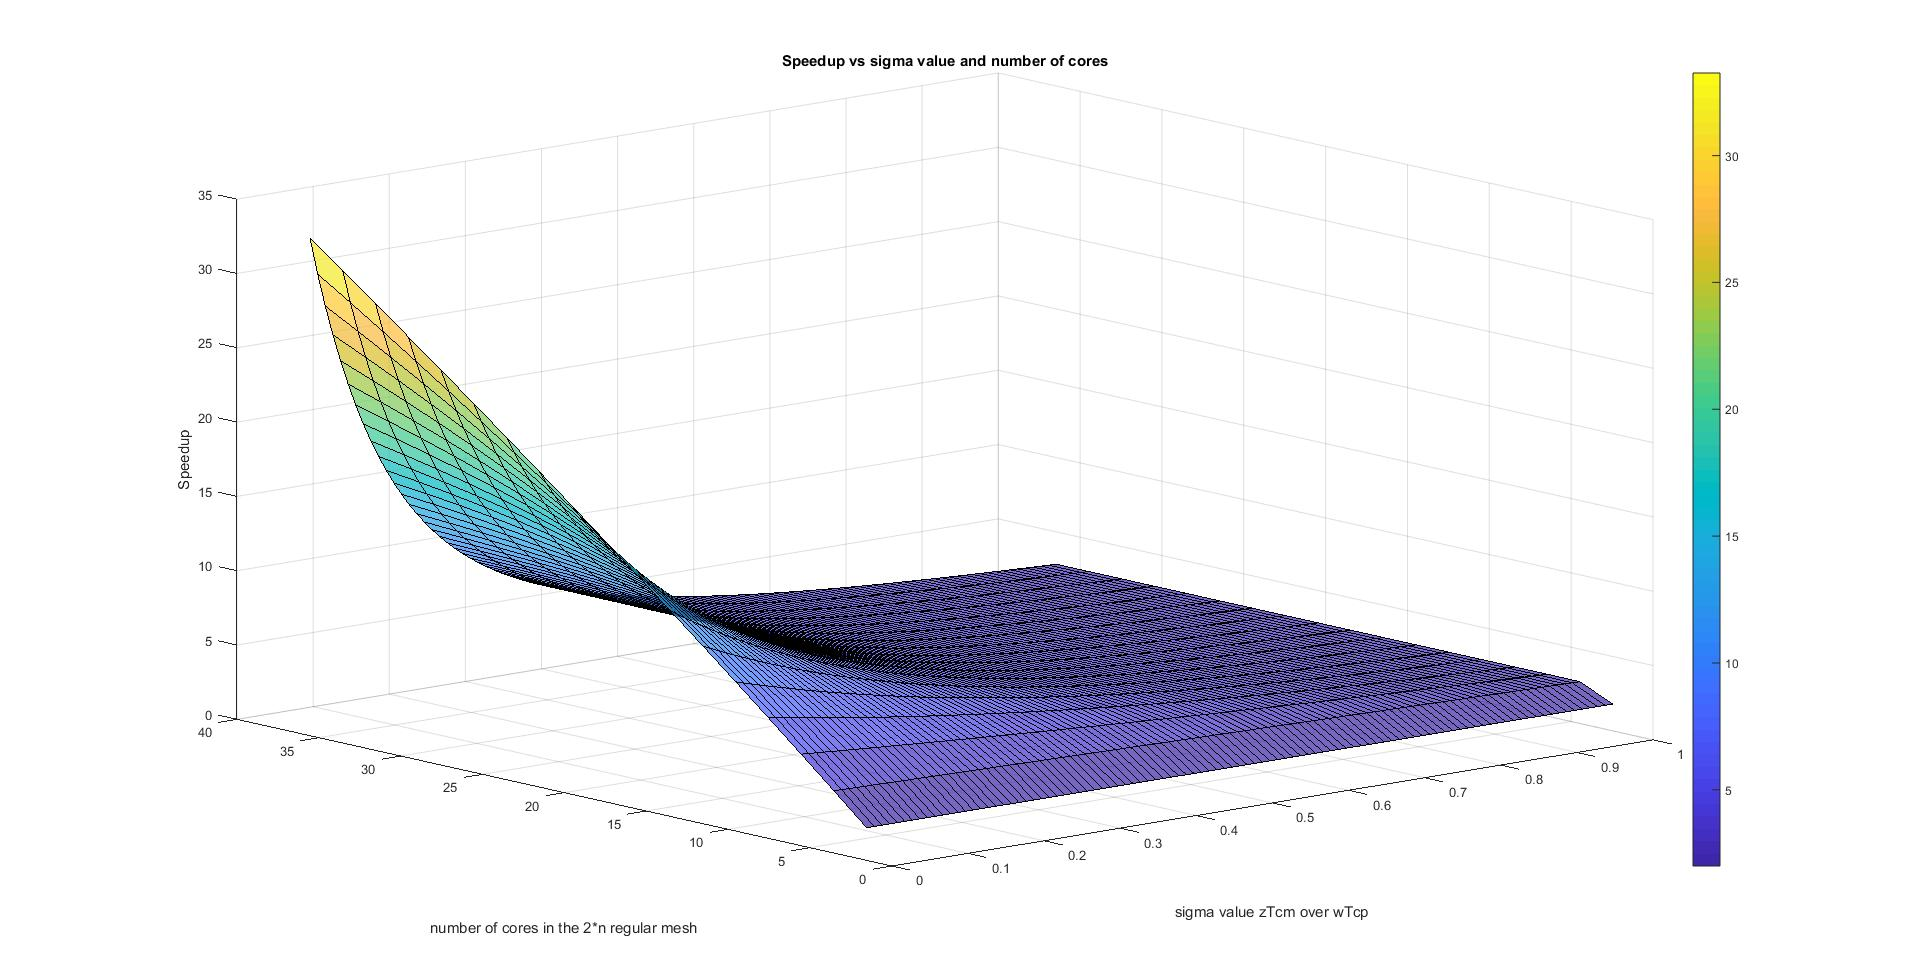
\includegraphics[width=0.85\linewidth]{figure/corner2n}
\caption{Speedup vs $\sigma$ value and number of cores in 2*n regular mesh}
\label{corner2n}
\end{figure}
\vspace*{30pt}

\begin{figure}[h]
\centering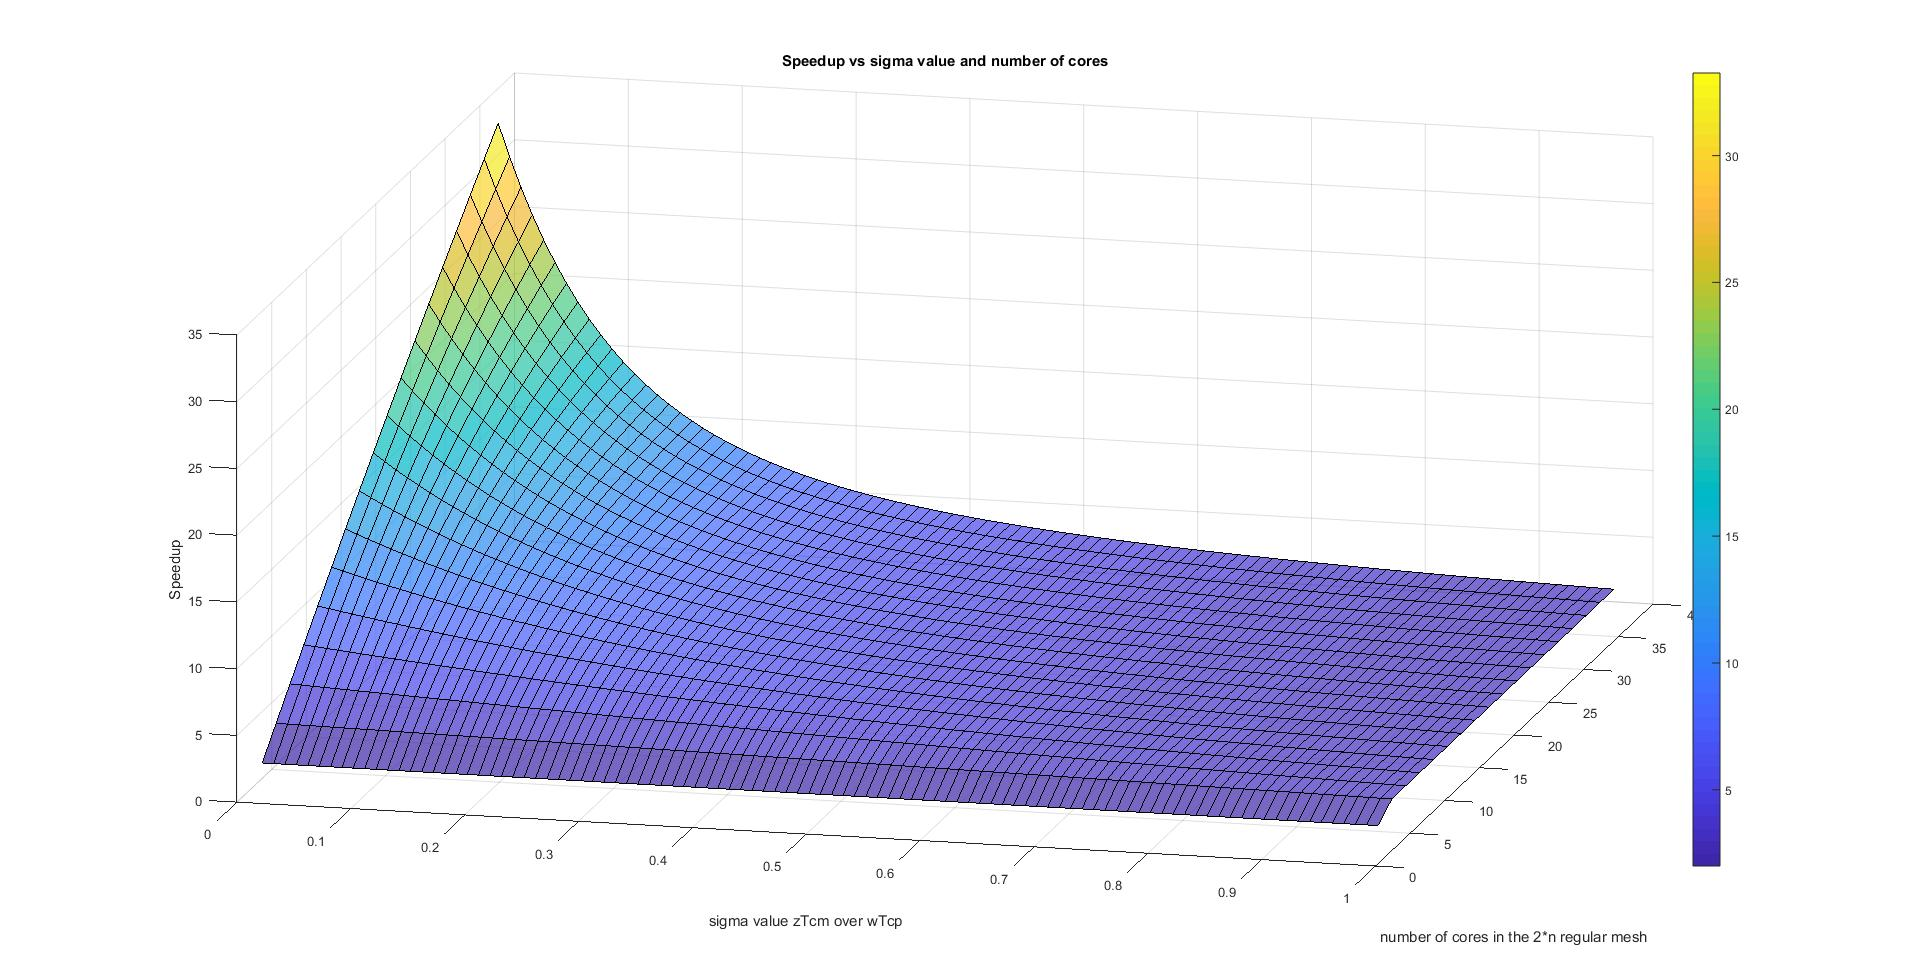
\includegraphics[width=0.85\linewidth]{figure/corner2n2}
\caption{Speedup vs $\sigma$ value and number of cores in 2*n regular mesh}
\label{corner2n2}
\end{figure}


\vspace*{30pt}

\subsubsection{3*n regular mesh simulation result}

Considering the $3*n $ regular mesh Fig .\ref{38f} Fig.\ref{bc3n},which represents the speedup vs the number of cores relationship as follows  Fig.\ref{corner3n}:

\begin{figure}[h]
\centering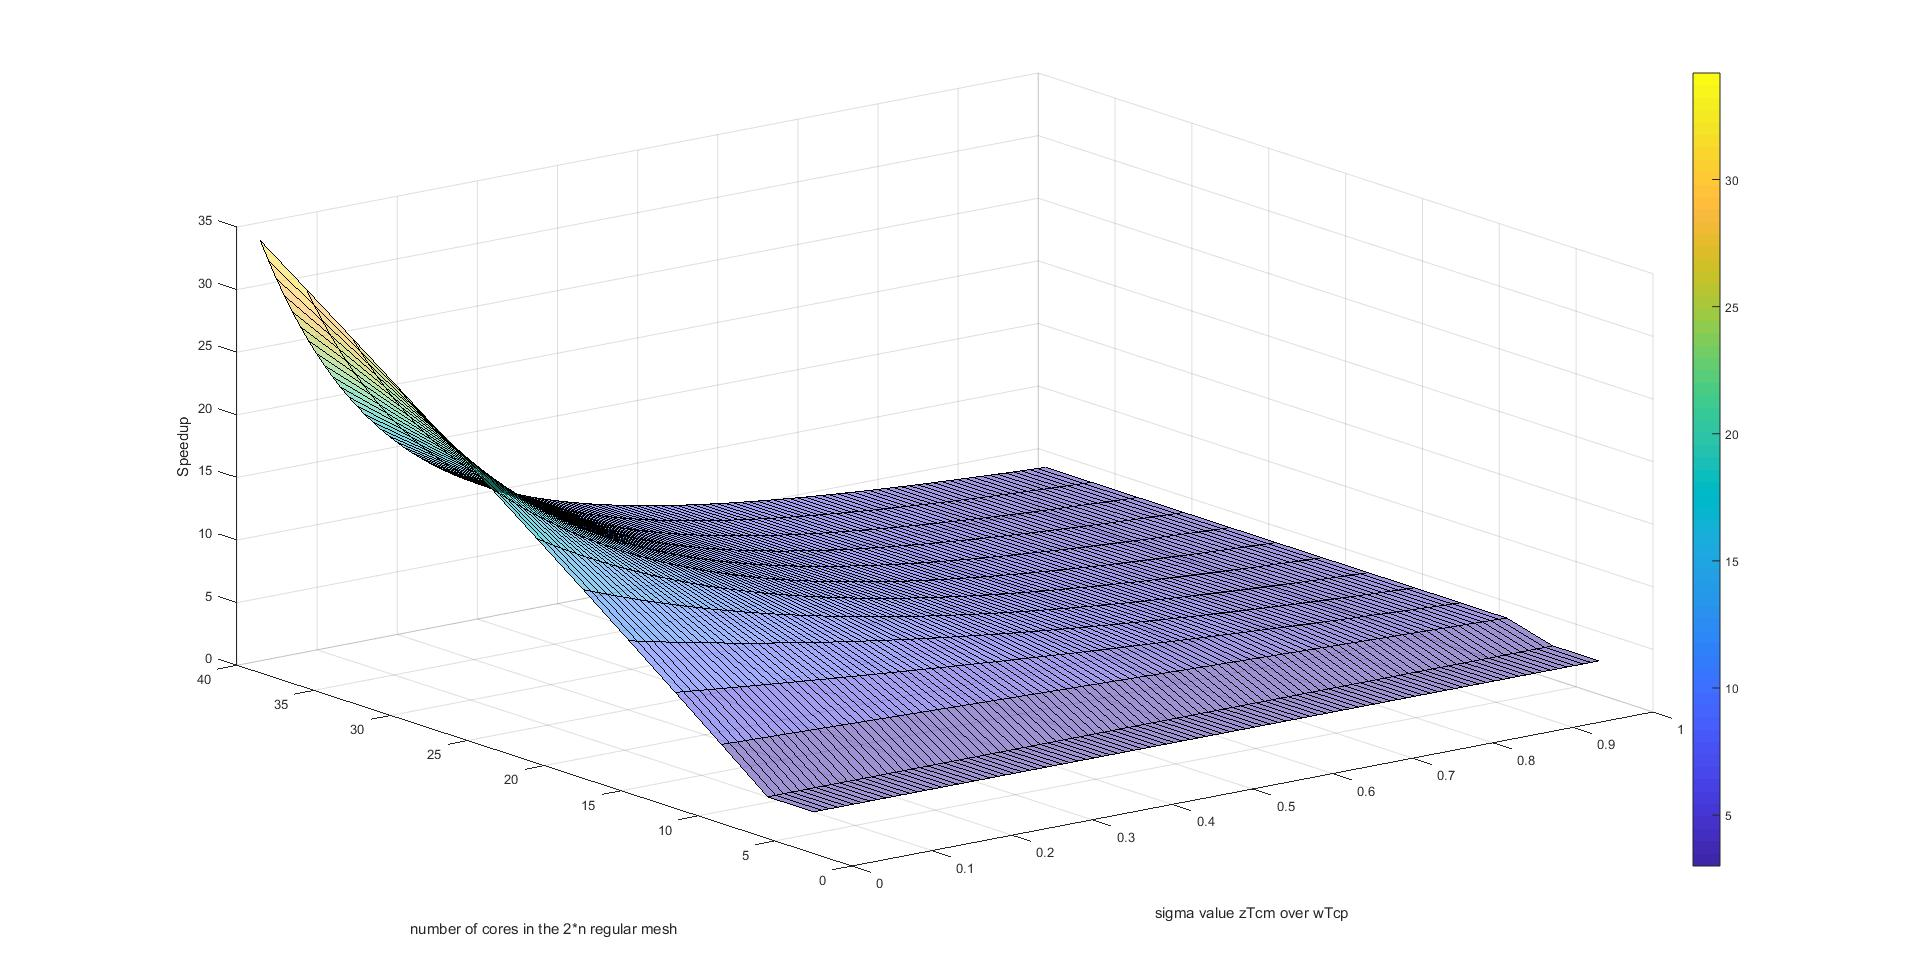
\includegraphics[width=0.85\linewidth]{figure/corner3n}
\caption{Speedup vs $\sigma$ value and number of cores in 3*n regular mesh}
\label{corner3n}
\end{figure}

\vspace*{50pt}

We can see from Fig.\ref{bc3n}. 

\begin{itemize}
\item If the $\sigma > 0.15$, the boundary data injection plan has positive speedup effect comparing with the corner injection plan. 
\item If the $\sigma <= 0.15$, the corner data injection plan will play a more helpful role.
\end{itemize}

\begin{figure}[h]
\centering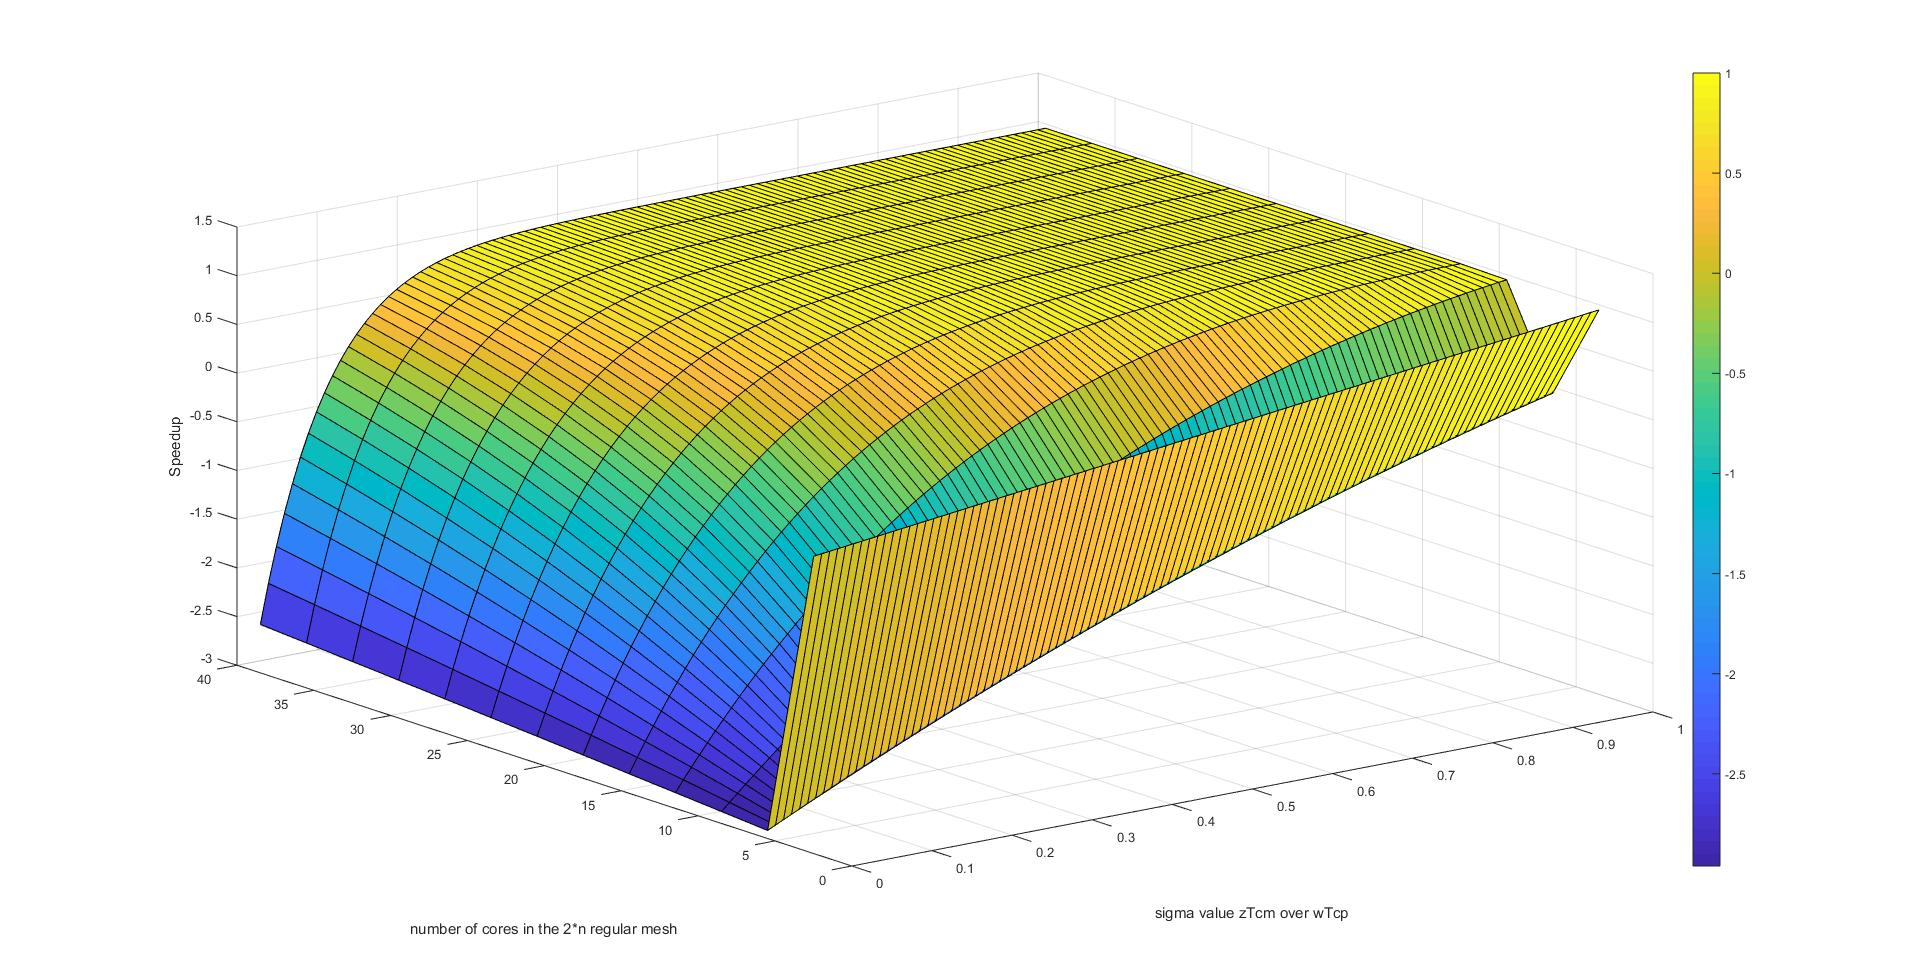
\includegraphics[width=0.85\linewidth]{figure/bc3n}
\caption{Speedup Difference between Corner and Boundary Data Injection in 3*n regular mesh}
\label{bc3n}
\end{figure}

\subsubsection{5*5 regular mesh inner grid simulation result}

Considering the $5*5$ regular mesh Fig .\ref{410f},which represents the speedup vs the number of cores relationship as follows:

The simulation result as follows Fig.\ref{inner4n}:

\begin{figure}[h]
\centering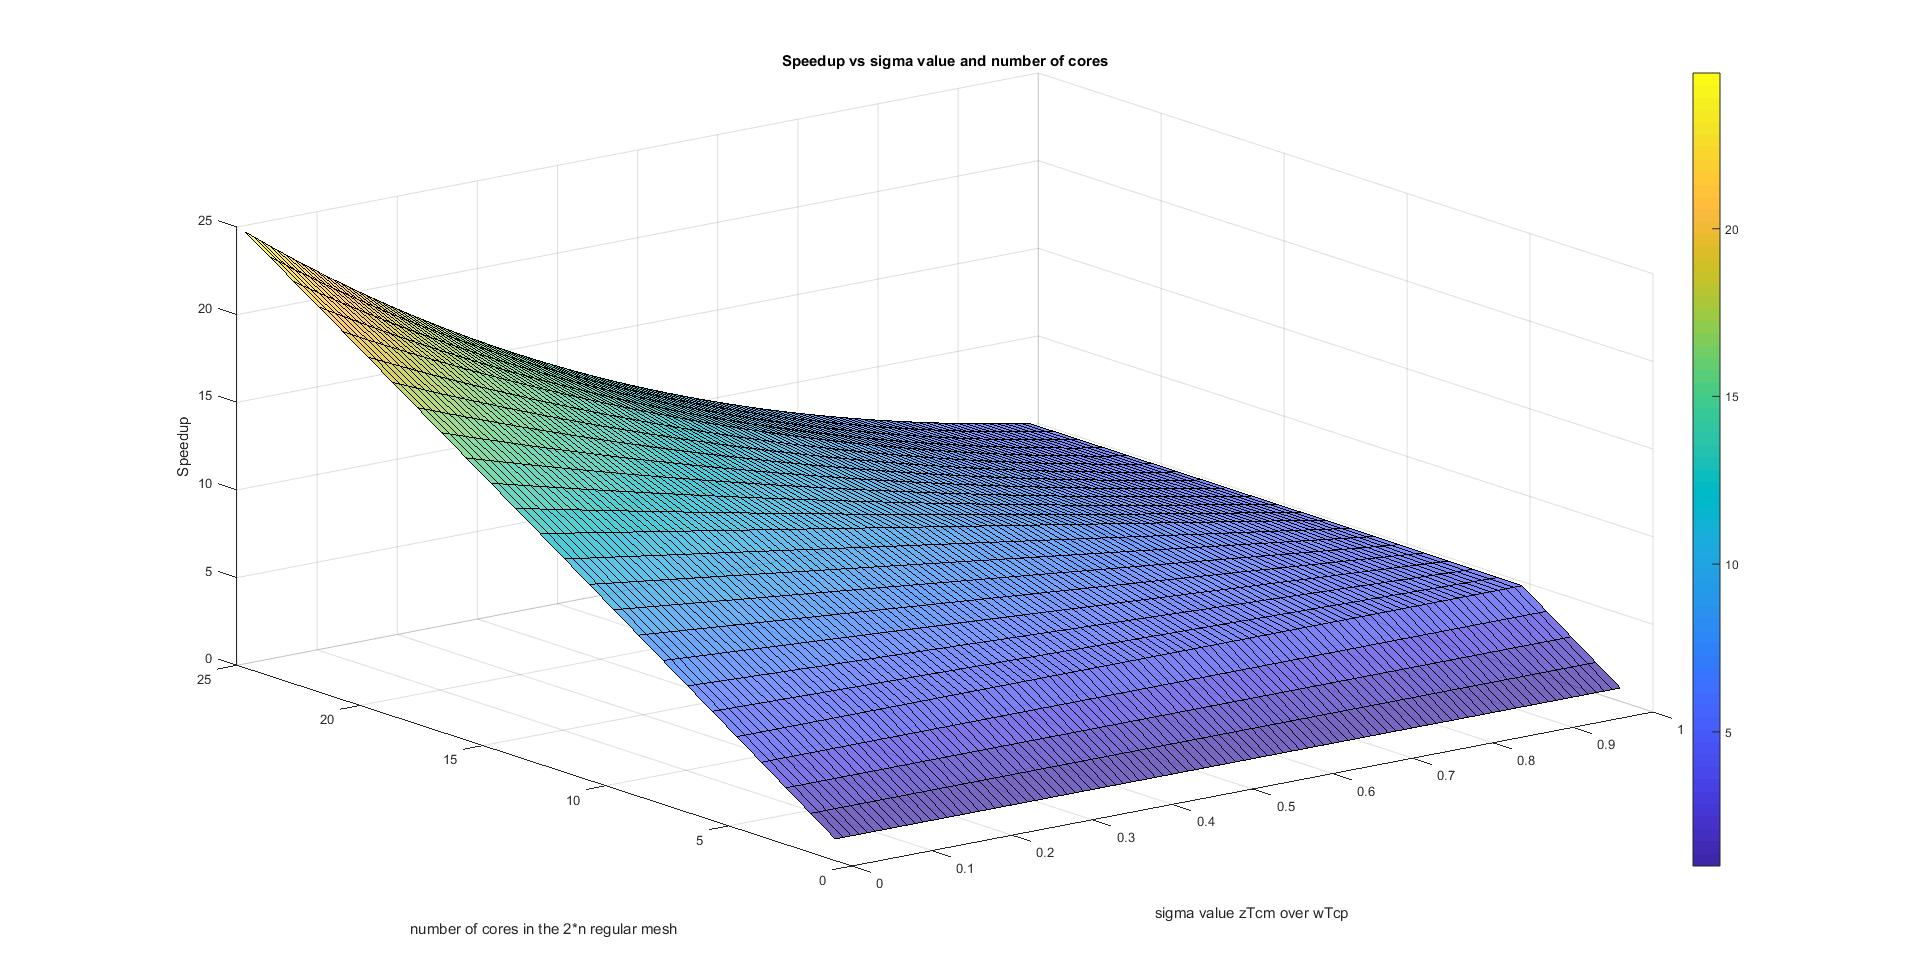
\includegraphics[width=0.85\linewidth]{figure/inner4n}
\caption{Speedup vs $\sigma$ value and number of cores in 4*n regular mesh}
\label{inner4n}
\end{figure}





\vspace*{50pt}
\subsection{Without Front End Schema}

\subsubsection{2*n regular mesh}
Considering the $2*n $ regular mesh Fig.\ref{210f}.The data injection position is on the corner.
\\
\vspace*{15pt}
The speedup vs the number of cores relationship as follows:

\begin{itemize}
\item we can see as the number of cores grows and the equal computational grow as well. 
\item At the same, the $\sigma$ value plays an import role, especially $\sigma > 0.25$. The speedup drops dramatically.
\end{itemize}


\begin{figure}[h]
\centering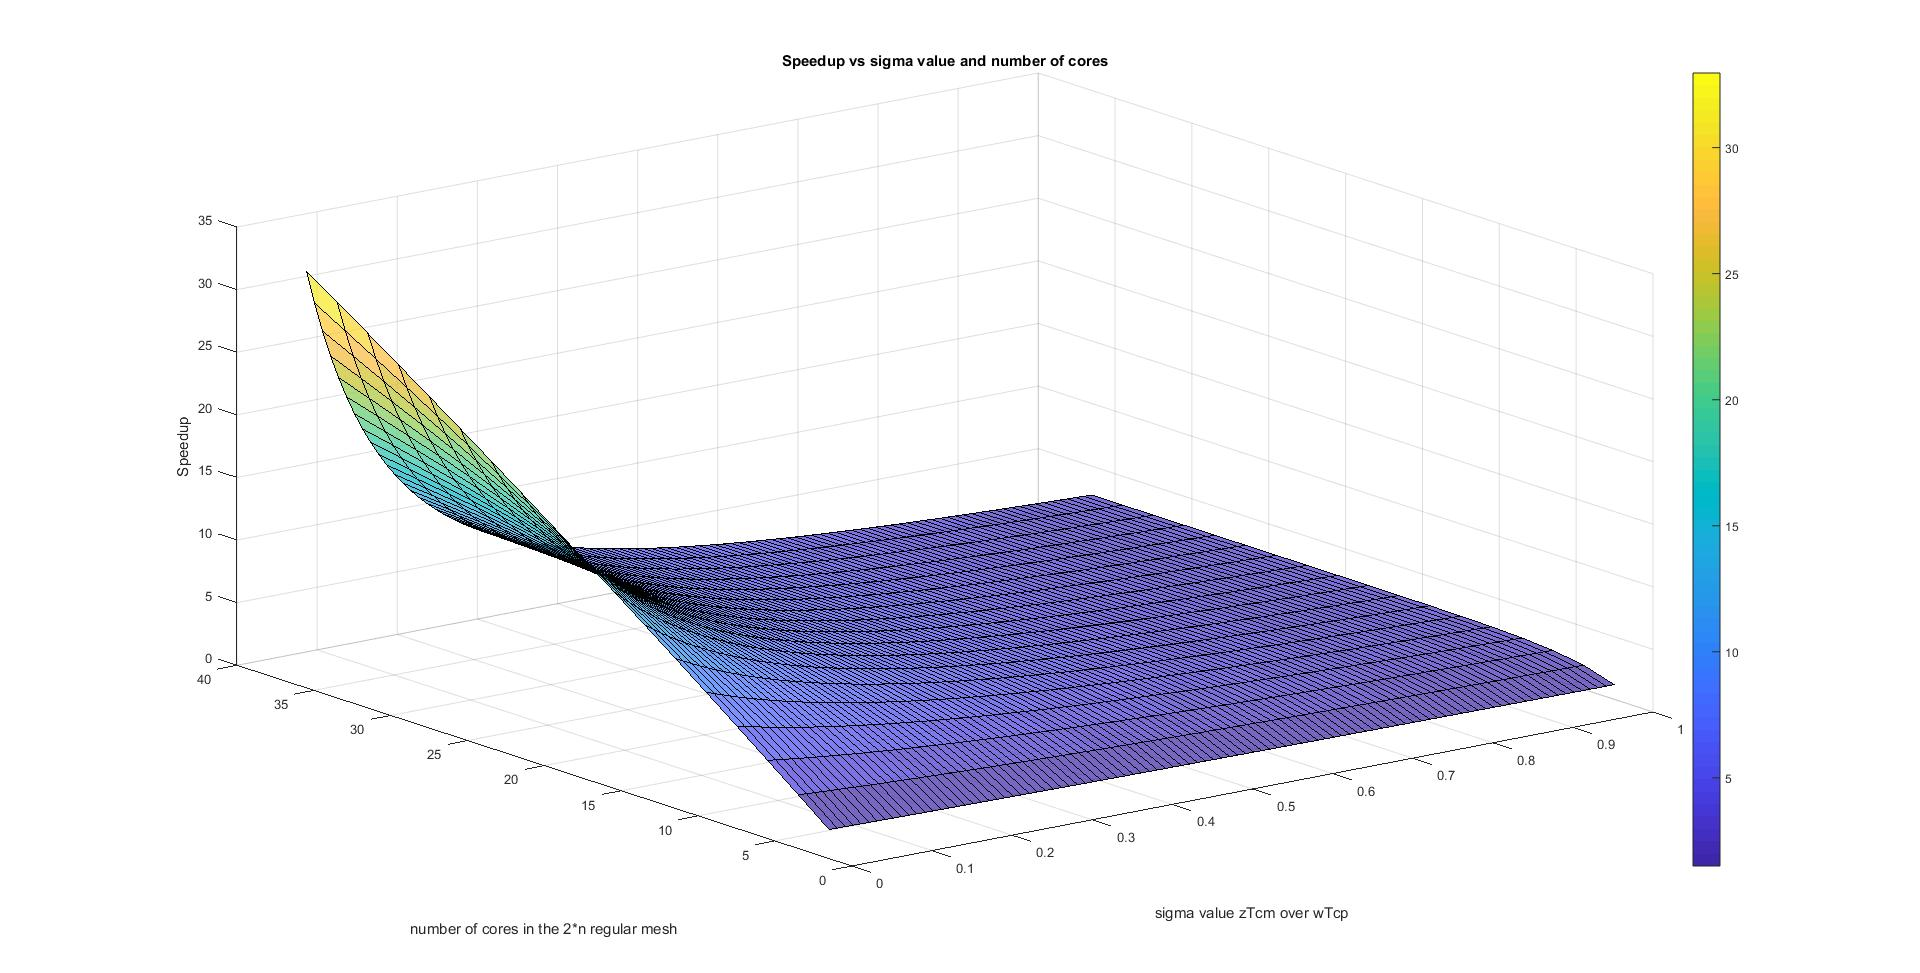
\includegraphics[width=0.85\linewidth]{figure/nocorner2n}
\caption{Speedup vs $\sigma$ value and number of cores in 2*n regular mesh}
\label{nocorner2n}
\end{figure}

\begin{figure}[h]
\centering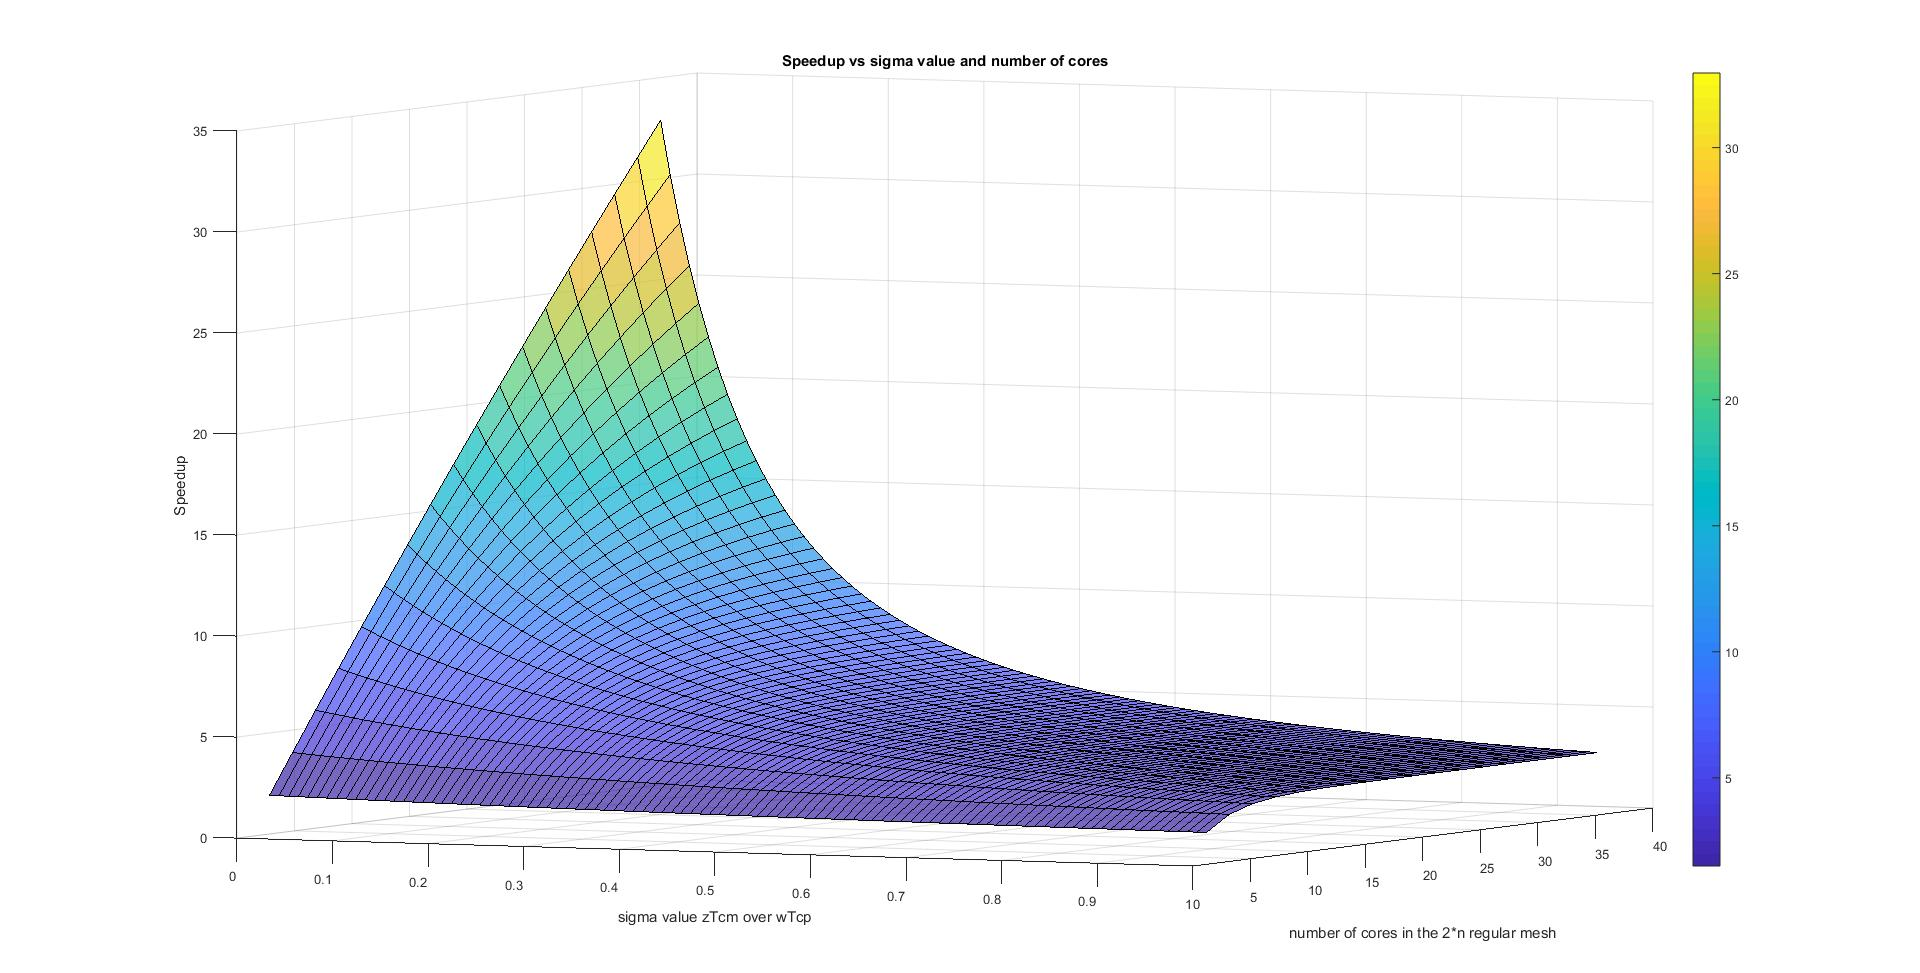
\includegraphics[width=0.85\linewidth]{figure/nocorner2n2}
\caption{Speedup vs $\sigma$ value and number of cores in 2*n regular mesh}
\label{nocorner2n2}
\end{figure}

\vspace*{50pt}

\subsubsection{3*n regular mesh simulation result}

Considering the $3*n $ regular mesh Fig.\ref{38f}.\\

The speedup vs the number of cores relationship as follows:

\begin{itemize}
\item If the $\sigma > 0.2$, the boundary data injection plan has positive speedup effect comparing with the corner injection plan. 
\item If the $\sigma <= 0.2$, the corner data injection plan will play a more helpful role.
\end{itemize}

\begin{figure}[h]
\centering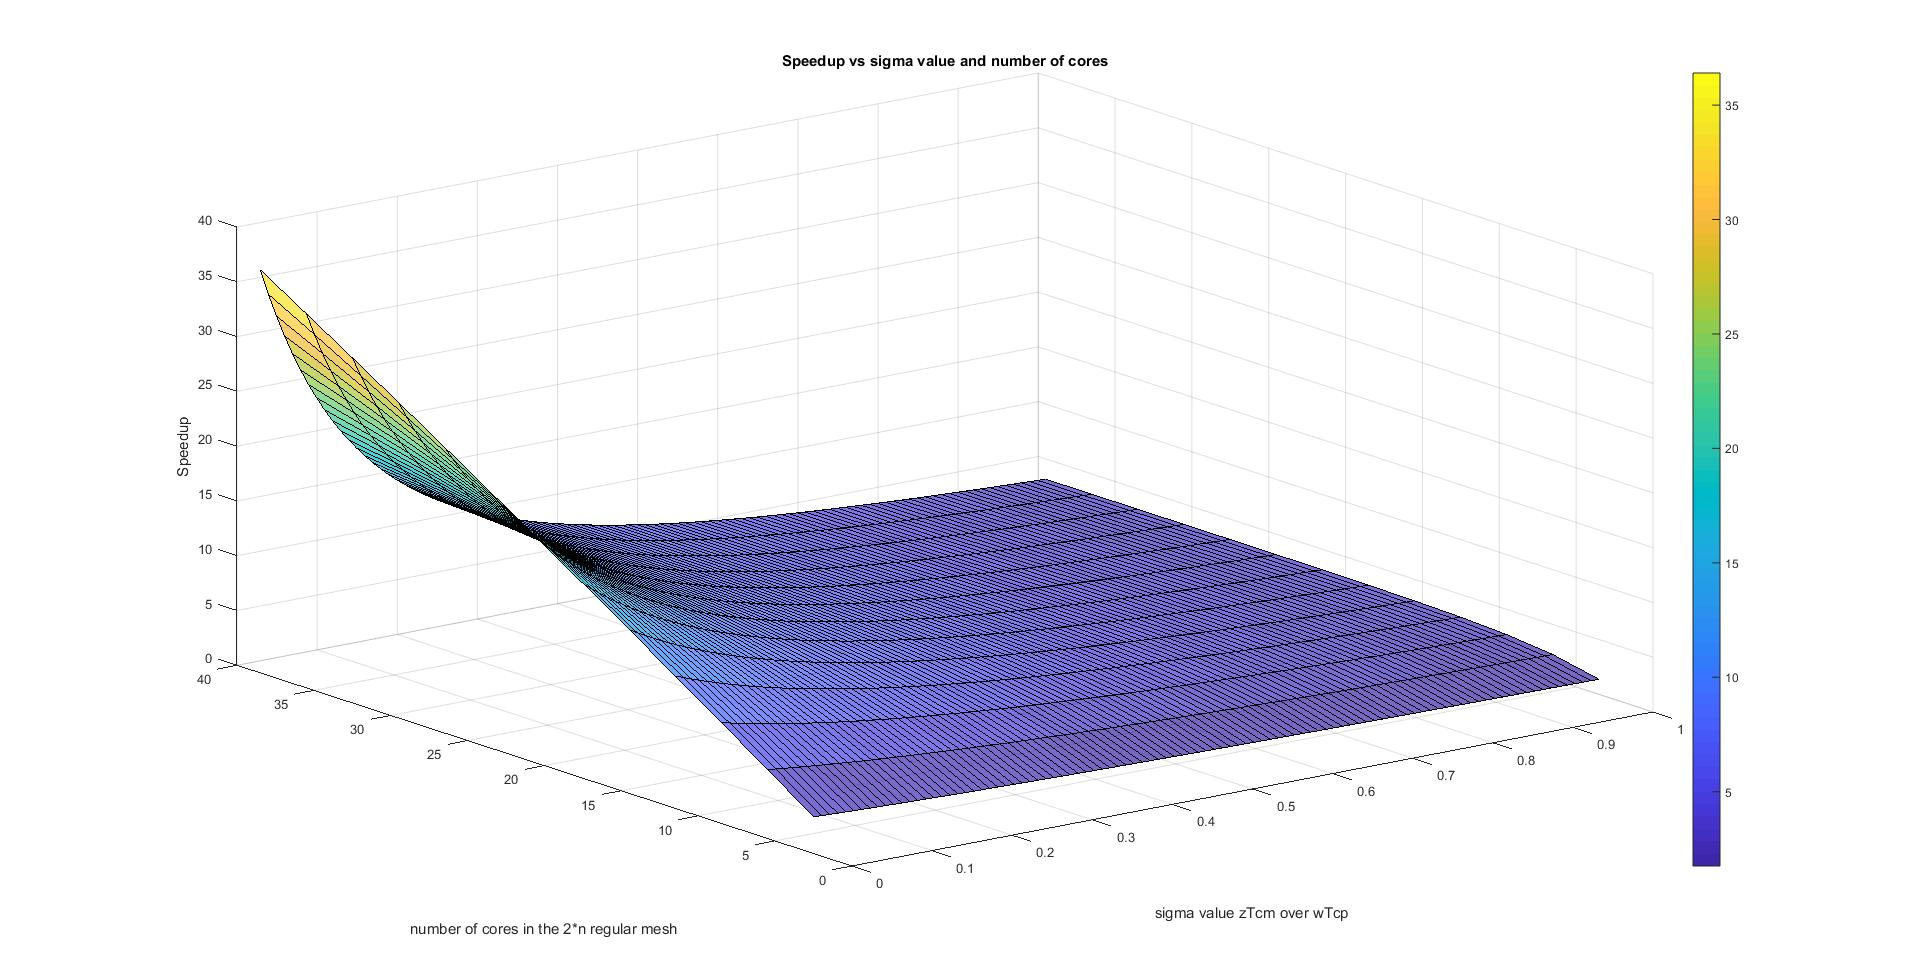
\includegraphics[width=0.85\linewidth]{figure/nocorner3n}
\caption{Speedup vs $\sigma$ value and number of cores in 3*n regular mesh}
\label{nocorner3n}
\end{figure}

\begin{figure}[h]
\centering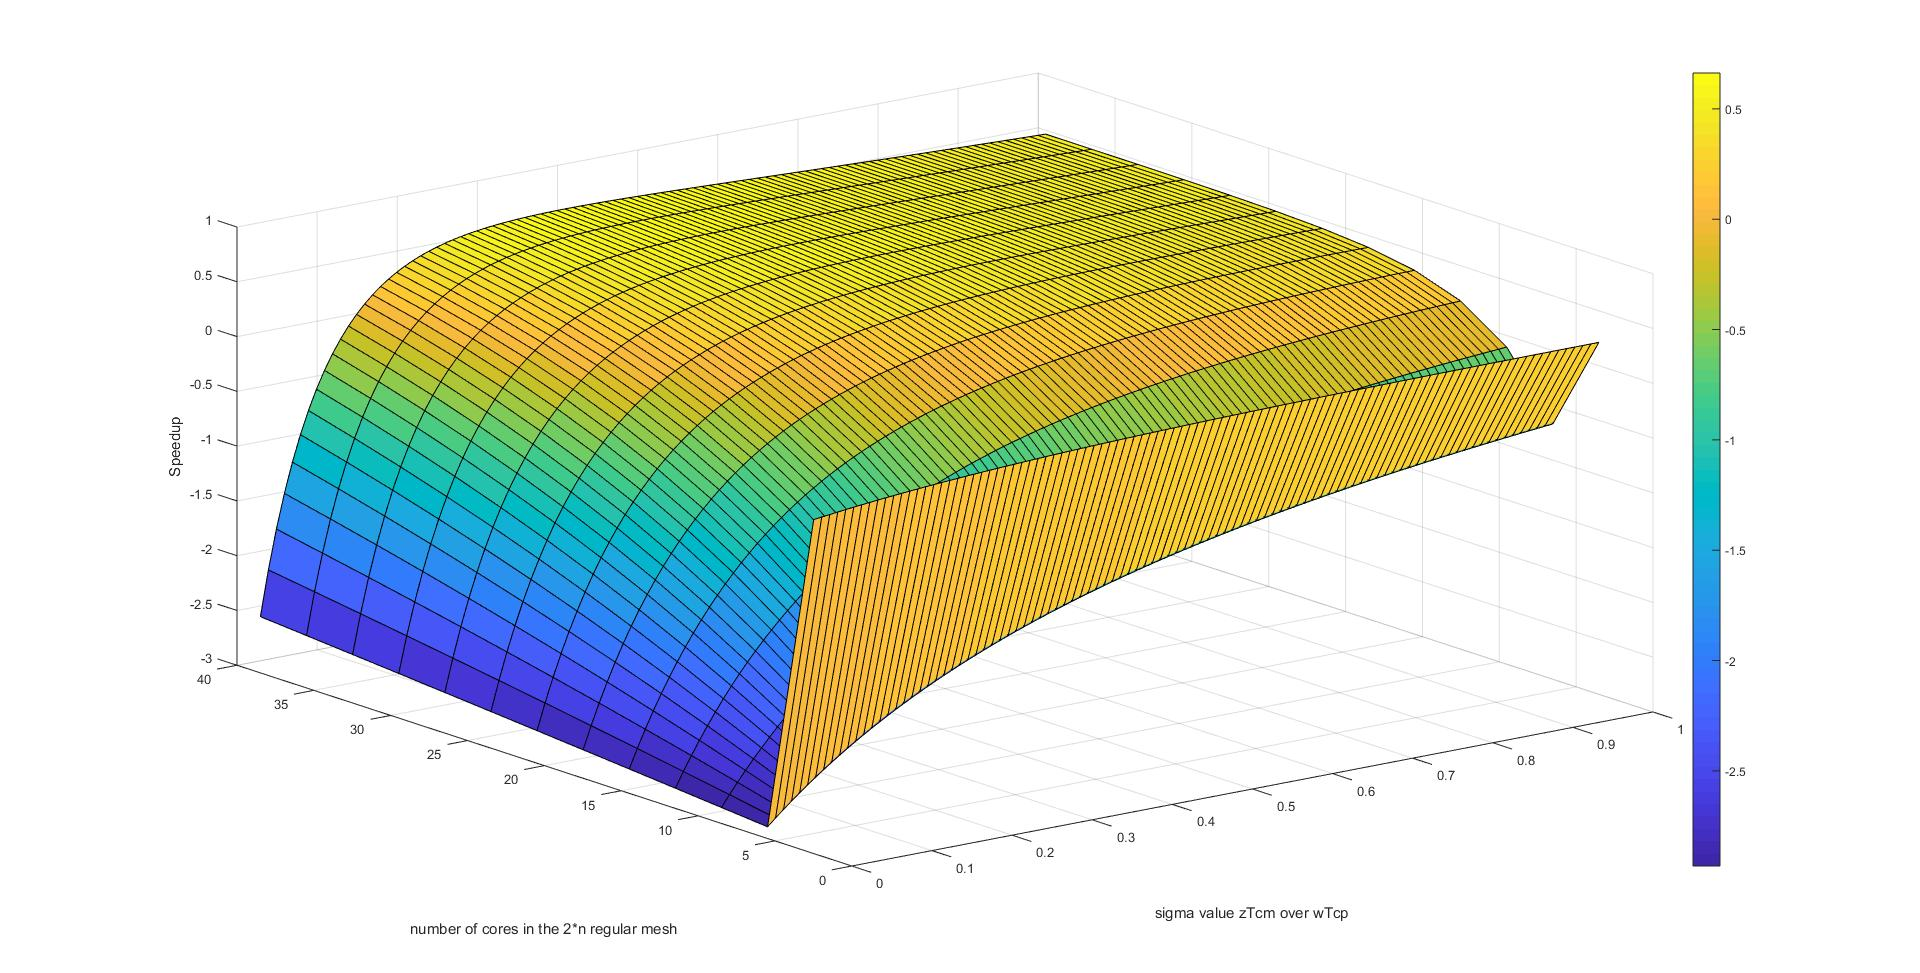
\includegraphics[width=0.85\linewidth]{figure/nobc3n}
\caption{Speedup Difference between Corner and Boundary Data Injection in 3*n regular mesh}
\label{nobc3n}
\end{figure}


\vspace*{50pt}
\subsubsection{5*5 regular mesh inner grid simulation result}
Considering the $5*5 $ regular mesh Fig.\ref{410f} and the data injection position is on the $position = 12$.
\\
The simulation result as follows Fig.\ref{noinner4n}:

\begin{figure}[h]
\centering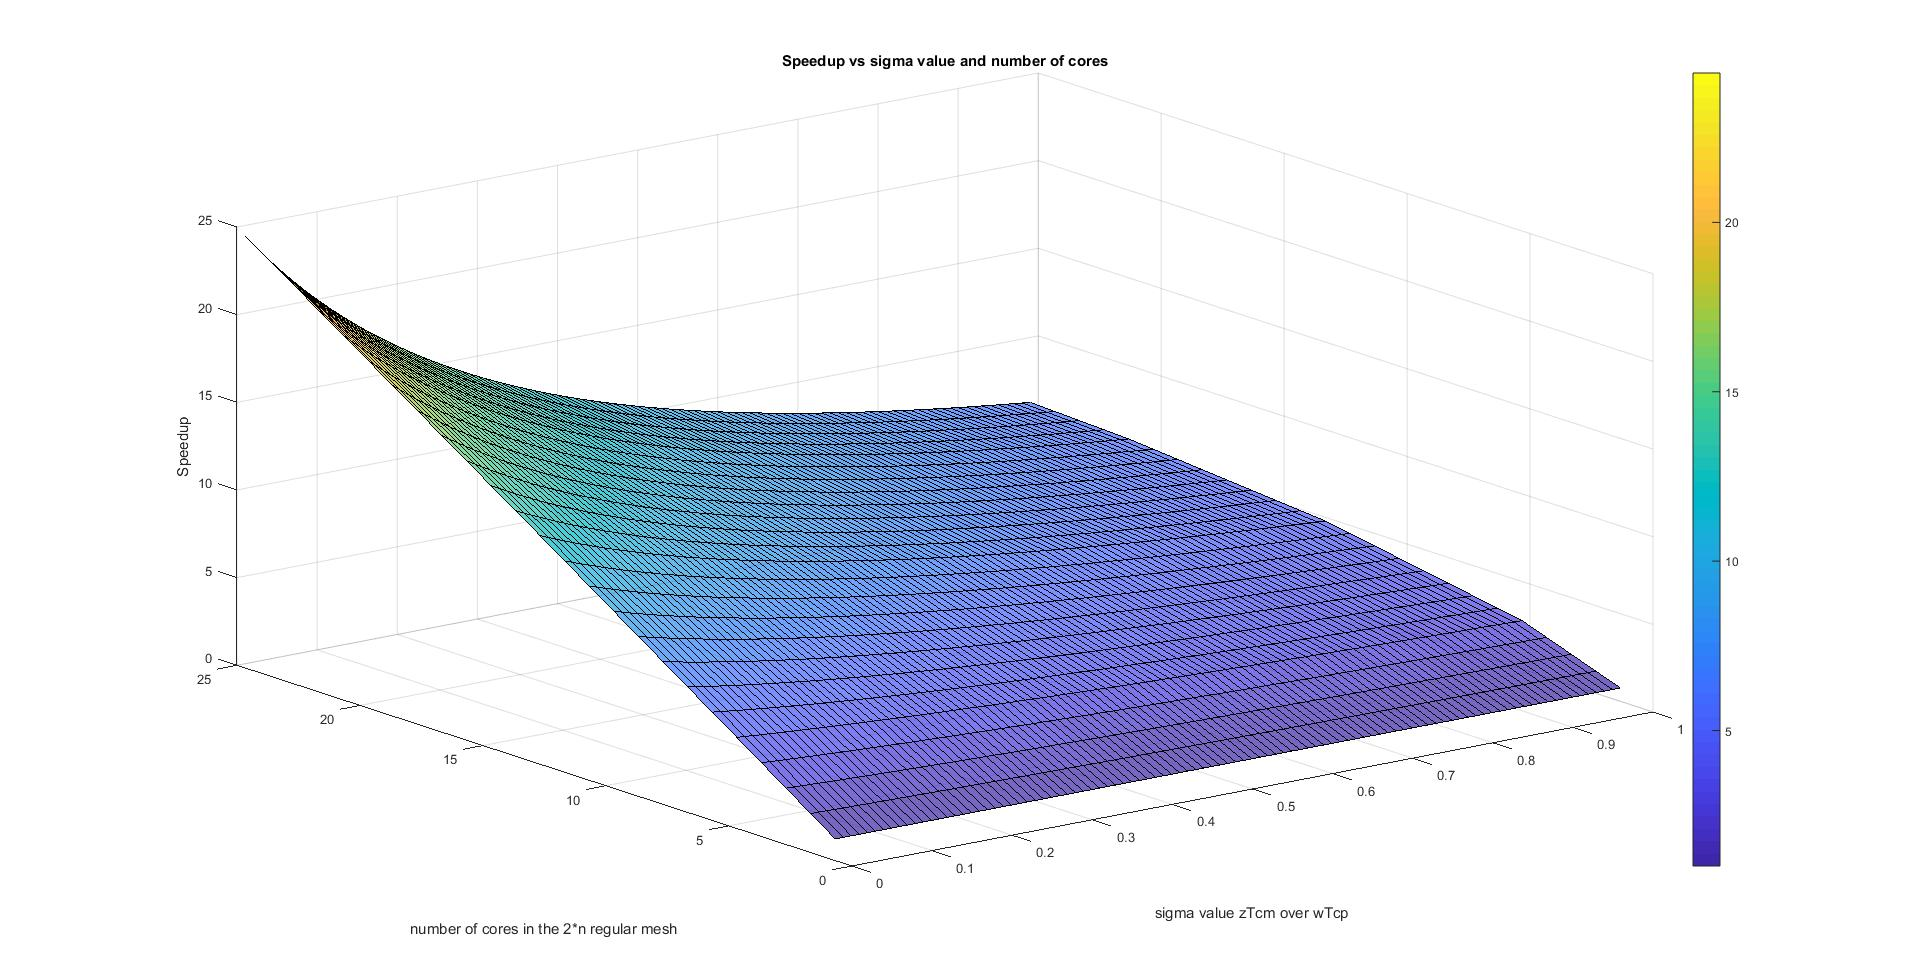
\includegraphics[width=0.85\linewidth]{figure/noinner4n}
\caption{Speedup vs $\sigma$ value and number of cores in 4*n regular mesh}
\label{noinner4n}
\end{figure}








\section{Re-balance Voronoi Diagram Multi-source load injection}

In this section, we introduce the Voronoi diagram technique to address the data injection position and data injection community division problem. 
\\
We will consider these problems from the following perspective:

\begin{itemize}
\item data load position dense or sparse
\item data load injection fraction even or different
\item how to choose data load injection position to achieve the high efficiency.
\end{itemize}

\subsection{General Case}

We use Manhattan Distance to divide the regular mesh area to Voronoi Cell \cite{fortune1987sweepline}.
\\
We can see the Fig.\ref{voronoi} shows the simulation result.

\begin{figure}[h]
\centering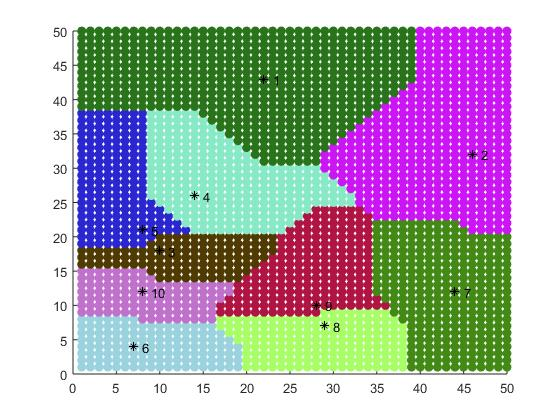
\includegraphics[width=0.8\linewidth]{figure/voronoi}
\caption{50*50 regular mesh with 10 data injection community division}
\label{voronoi}
\end{figure}

\vspace*{50pt}

\subsection{Data Injection Position Dense}
If the data injection positions are dense, which means the data injection position connect with each other. 

\vspace*{15pt}

The sun-optimal solution is that

\begin{itemize}
\item we consider the whole cluster data load injection as one data injection 
\item execute the equal power algorithm in chapter one to process the divisible load theory principle.
\item re-balance the load fraction between nodes in the cluster
\end{itemize}

Consider the Fig.\ref{dense1}

\vspace*{15pt}

\begin{figure}[h]
\centering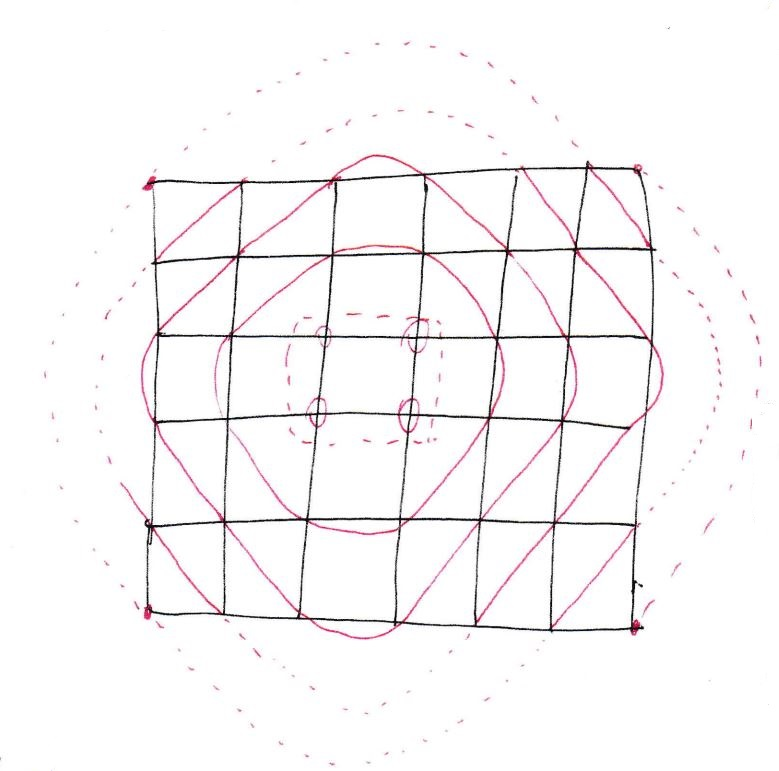
\includegraphics[width=0.8\linewidth]{figure/dense1}
\caption{4 data injection connecting with each other consists of a whole cluster}
\label{dense1}
\end{figure}

The equal power matrix with front end as follows:

\begin{equation}
{
\left[ \begin{array}{ccccc}
4 & 8 & 10 & 6 & 2 \\
1 & -1 & 0 & 0 & 0\\
0 & \sigma -1 & 1 & 0 & 0  \\
0 & \sigma -1 & \sigma & 1 & 0  \\
0 & \sigma -1 & \sigma & \sigma & 1  \\
\end{array} 
\right ]}  
\end{equation}


The equal power matrix without front end as follows:

\begin{equation}
{
\left[ \begin{array}{ccccc}
4 & 8 & 10 & 6 & 2 \\
1 & {\sigma}^{\star} & 0 & 0 & 0 \\
1 & -\sigma & {\sigma}^{\star} & 0 & 0  \\
1 & -\sigma & -\sigma & {\sigma}^{\star} & 0  \\
1 & -\sigma & -\sigma & -\sigma & {\sigma}^{\star}\\

\end{array} 
\right ]} 
\end{equation}

\vspace*{50pt}

Consider the Fig.\ref{dense2}
\begin{figure}[h]
\centering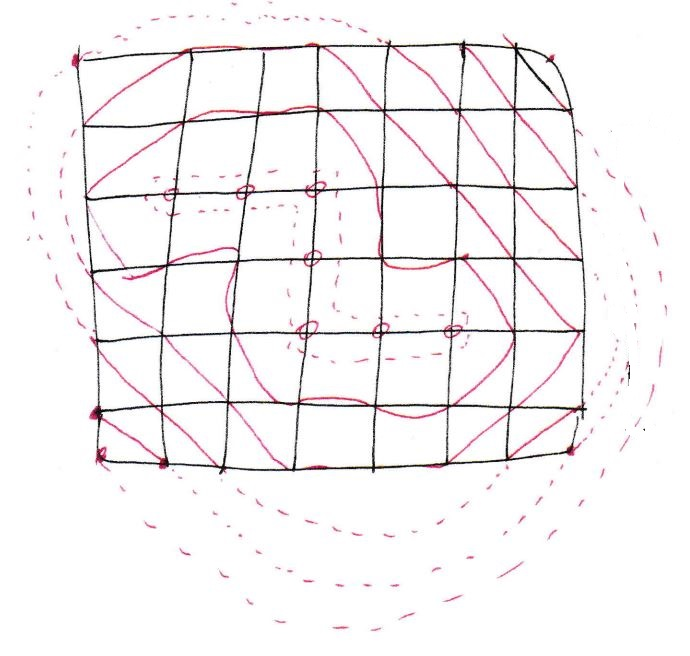
\includegraphics[width=0.8\linewidth]{figure/dense2}
\caption{7 data injection connecting with each other consist of a whole cluster}
\label{dense2}
\end{figure}

\vspace*{20pt}
The equal power matrix with front end as follows:

\begin{equation}
{
\left[ \begin{array}{ccccccc}
7 & 14 & 15 & 10 & 6 & 3 & 1 \\
1 & -1 & 0 & 0 & 0 & 0 & 0\\
0 & \sigma -1 & 1 & 0 & 0 & 0 & 0 \\
0 & \sigma -1 & \sigma & 1 & 0 & 0 & 0 \\
0 & \sigma -1 & \sigma & \sigma & 1 & 0 & 0 \\
0 & \sigma -1 & \sigma & \sigma & \sigma & 1 & 0 \\
0 & \sigma -1 & \sigma & \sigma & \sigma & \sigma & 1 \\
\end{array} 
\right ]}  
\end{equation}

\vspace*{20pt}
The equal power matrix without front end as follows:

\begin{equation}
{
\left[ \begin{array}{ccccccc}
7 & 14 & 15 & 10 & 6 & 3 & 1 \\
1 & {\sigma}^{\star} & 0 & 0 & 0 & 0 & 0 \\
1 & -\sigma & {\sigma}^{\star} & 0 & 0 & 0 & 0 \\
1 & -\sigma & -\sigma & {\sigma}^{\star} & 0 & 0 & 0 \\
1 & -\sigma & -\sigma & -\sigma & {\sigma}^{\star} & 0 & 0\\
1 & -\sigma & -\sigma & -\sigma & -\sigma & {\sigma}^{\star}  & 0\\
1 & -\sigma & -\sigma & -\sigma & -\sigma & -\sigma & {\sigma}^{\star}\\

\end{array} 
\right ]} 
\end{equation}

So this kind of problem is transfered to finding the number of node on each level(contour line).

\vspace*{50pt}
\subsection{Choosing The Data Load Position}
The data injection position are affected by two factors. 

\begin{itemize}
\item the distance between each data load injection
\item the number of unit cores in its Voronoi cell community.
\end{itemize}

So we choose the Manhattan distance centroidal voronoi tessellations\cite{du1999centroidal} to choose the data injection position.
\\
For example, we consider the 80*80 regular mesh, we have 10 data injection budget to choose 10 appropriate position.

We can see the simulation result from Fig.\ref{cvt1} and Fig.\ref{cvt20}
\vspace*{20pt}

\begin{figure}[h]
\centering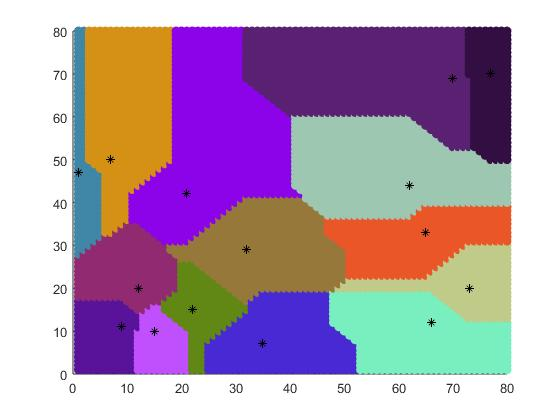
\includegraphics[width=0.8\linewidth]{figure/cvt1}
\caption{Random choose 10 potential position to do the community division }
\label{cvt1}
\end{figure}

\begin{figure}[h]
\centering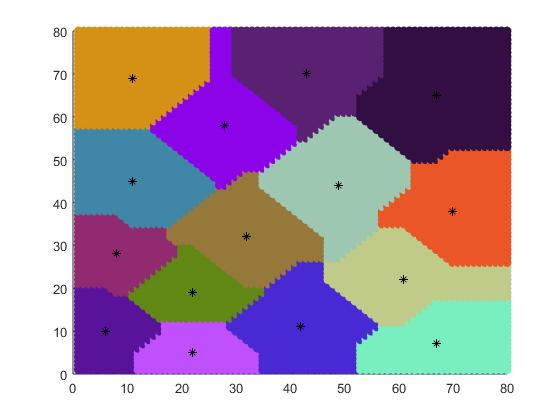
\includegraphics[width=0.8\linewidth]{figure/cvt20}
\caption{After 20 rounds the division achieve stable}
\label{cvt20}
\end{figure}

\subsection{Re-balance the community division }

Considering the speedup ability depends on the number of short distance unit core.
So after $1000$ times random experiment, we find we can achieve the same computation ability yet save over $30\%$ unit core.

\vspace*{20pt}
\textbf{
The principle is we choose the minimum value of the largest depth of each community as the depth rule.}

$$L =  min(max(voronoi \quad cell \quad depth))$$

\vspace*{20pt}

One example Fig.\ref{voronoi} Fig.\ref{voronoisave} presents:
\\

\begin{figure}[h]
\centering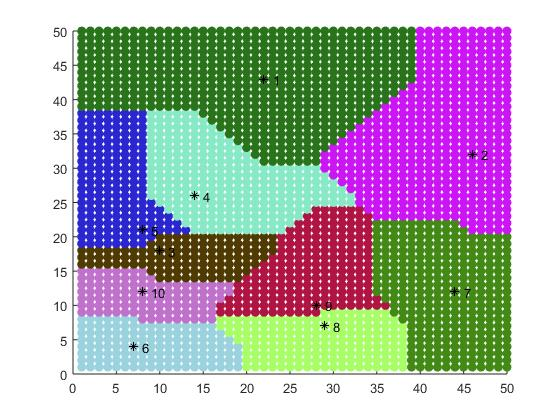
\includegraphics[width=0.8\linewidth]{figure/voronoi}
\caption{50*50 regular mesh with 10 division cell}
\label{voronoi}
\end{figure}

\begin{figure}[h]
\centering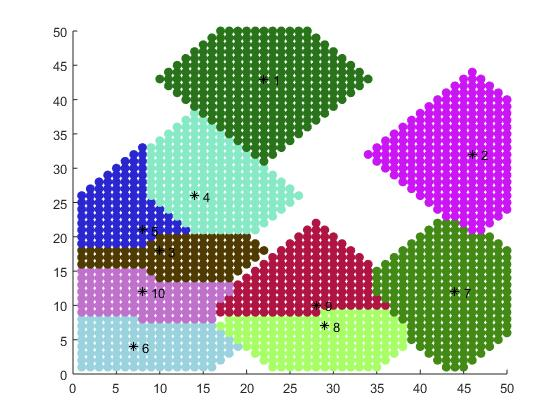
\includegraphics[width=0.8\linewidth]{figure/voronoisave}
\caption{50*50 regular mesh with 10 division cell and save over 30\% unit core}
\label{voronoisave}
\end{figure}

We also can find the speedup result from figures Fig.\ref{voronoicurve} and Fig.\ref{voronoisavecurve}:
\\
\begin{itemize}
\item $\sigma < 0.2$ the ratio is $5$. Fig.\ref{voronoicurve}
\item after re-balance the ratio is about $2.7$ \ref{voronoisavecurve}
\end{itemize}

\begin{figure}[h]
\centering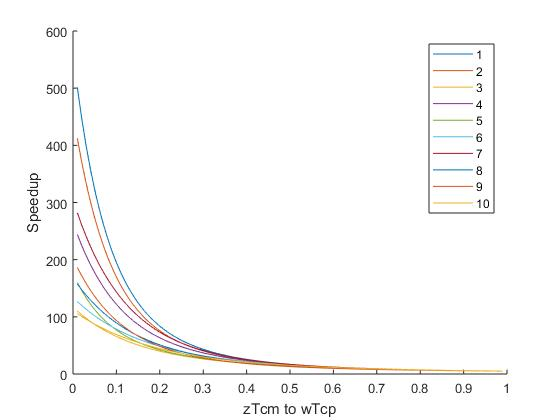
\includegraphics[width=0.8\linewidth]{figure/voronoi_curve}
\caption{50*50 regular mesh with 10 division cell}
\label{voronoicurve}
\end{figure}

\begin{figure}[h]
\centering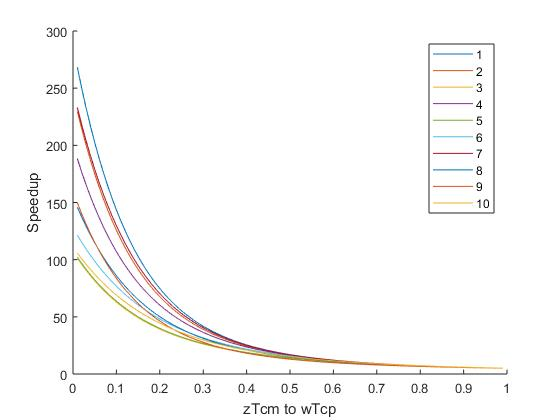
\includegraphics[width=0.8\linewidth]{figure/voronoi_curve2}
\caption{50*50 regular mesh with 10 division cell}
\label{voronoisavecurve}
\end{figure}

















\section{Optimal Mass Transport}

In this section,we extend the optimal mass transport theory algorithm framework \cite{gu2013variational} \cite{su2017volume} to address the data injection division problem. 

\vspace*{20pt}

The original method depends on the rigorous geometry structure,yet in the real application,the implementation is hard and not stable because of the numerical calculation errors. \\

I re-implement this framework using Monte Carlo method, which can be extend to $N$ dimension. In addition, the implement is simple and we get the appropriate accurate effect as adding more sampling points.
\\

Let's consider two situations as example.
\begin{itemize}
\item Given an initial division,try to redivide the regular mesh to even division using the minimum cost. For example, the number of unit core ratio of 10 pieces is [0.4 0.4 0.4 0.4 0.4 0.4 0.4 0.4 0.4 0.4]
\item Give an initial division,try to redivide the regular mesh to a target measure division using the minimum cost.For example,the number of unit core ratio of 10 pieces is [0.4 0.3 0.3 0.4 0.2 0.2 0.3 0.4 0.7 0.9]
\end{itemize}



\subsection{Situation 1}

The initial division as follows Fig.\ref{voronoiinit}:

\begin{figure}[h]
\centering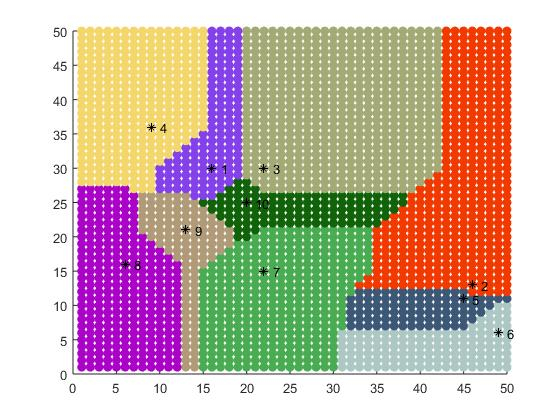
\includegraphics[width=0.8\linewidth]{figure/voronoiinit}
\caption{50*50 regular mesh with 10 data injection community division}
\label{voronoiinit}
\end{figure}

\vspace*{30pt}
The optimal mass transport even division as follows Fig.\ref{omtcell}:

\begin{figure}[h]
\centering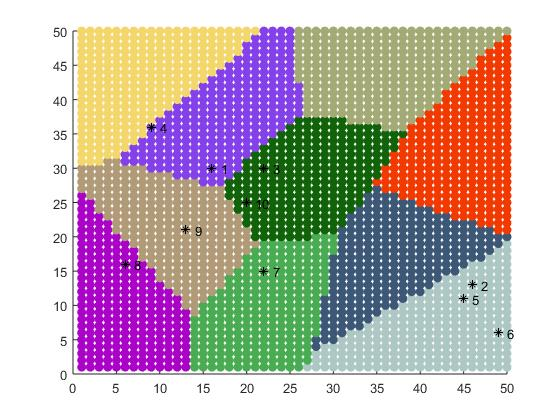
\includegraphics[width=0.8\linewidth]{figure/omtcell}
\caption{50*50 regular mesh with 10 data injection community division}
\label{omtcell}
\end{figure}
\vspace*{30pt}

After re-choose the data injection position as follows Fig.\ref{omtcell2}:
\begin{figure}[h]
\centering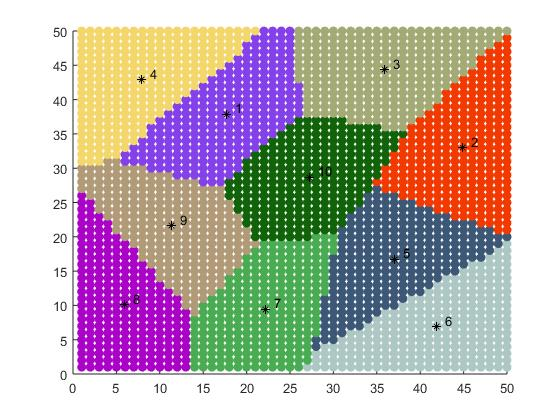
\includegraphics[width=0.8\linewidth]{figure/omtcell2}
\caption{50*50 regular mesh with 10 data injection community division}
\label{omtcell2}
\end{figure}

\vspace*{30pt}

The speedup ratio as follows:\\

The initial speedup figure. Fig.\ref{voronoicurve}
\\

\begin{figure}[h]
\centering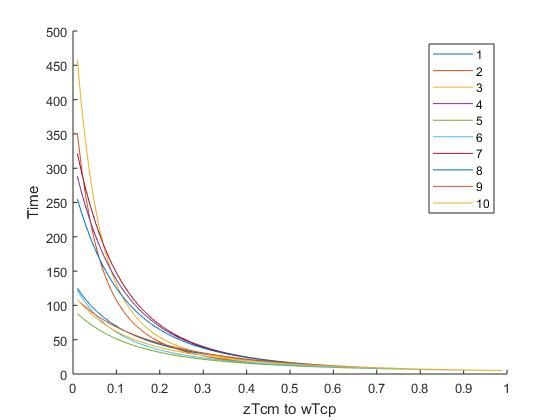
\includegraphics[width=0.8\linewidth]{figure/voronoicurve}
\caption{Speedup vs $\sigma$ in different community division}
\label{voronoicurve}
\end{figure}


Re-balance optimize speedup figure Fig.\ref{voronoicurve2}
\\

\begin{figure}[h]
\centering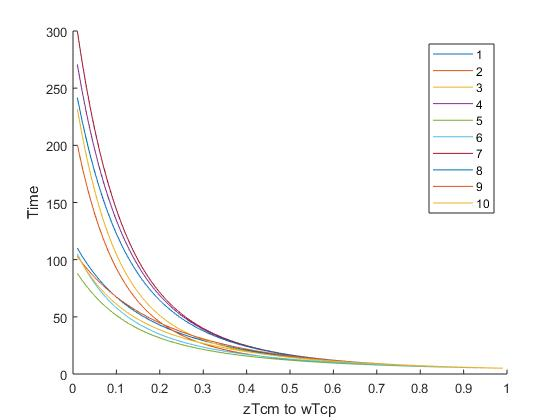
\includegraphics[width=0.8\linewidth]{figure/voronoicurve2}
\caption{Speedup vs $\sigma$ in different community division}
\label{voronoicurve2}
\end{figure}


The optimal mass transport speedup figure Fig.\ref{voronoicurve3}
\\

\begin{figure}[h]
\centering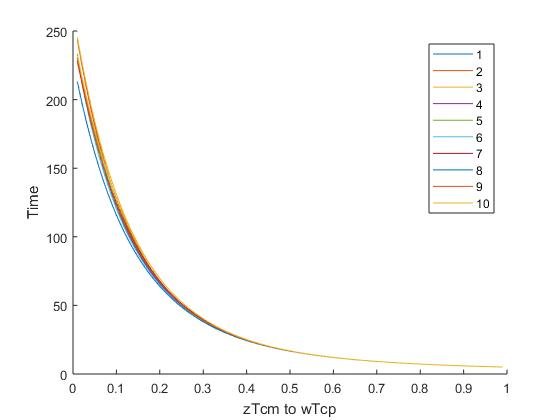
\includegraphics[width=0.8\linewidth]{figure/voronoicurve3}
\caption{Speedup vs $\sigma$ in different community division}
\label{voronoicurve3}
\end{figure}

\subsection{Situation 2}

\begin{figure}[h]
\centering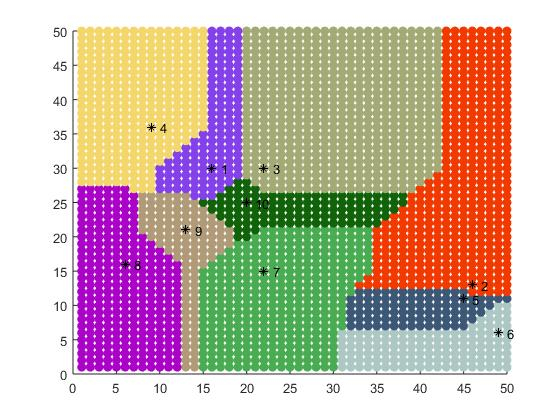
\includegraphics[width=0.8\linewidth]{figure/voronoiinit}
\caption{50*50 regular mesh with 10 data injection community division}
\label{voronoiinit}
\end{figure}

The optimal mass transport even division as follows:
\\

\begin{figure}[h]
\centering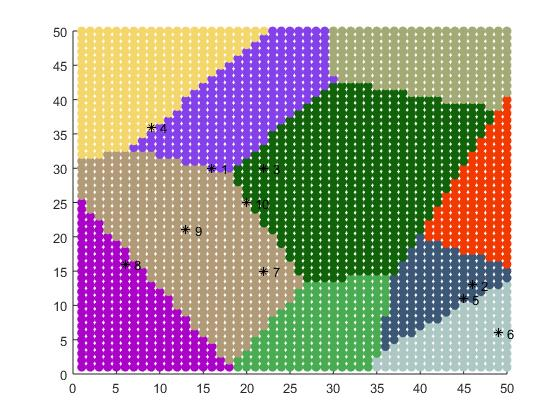
\includegraphics[width=0.8\linewidth]{figure/2omtcell}
\caption{50*50 regular mesh with 10 data injection community division}
\label{2omtcell}
\end{figure}

After re-choose the data injection position as follows:
\\
\begin{figure}[h]
\centering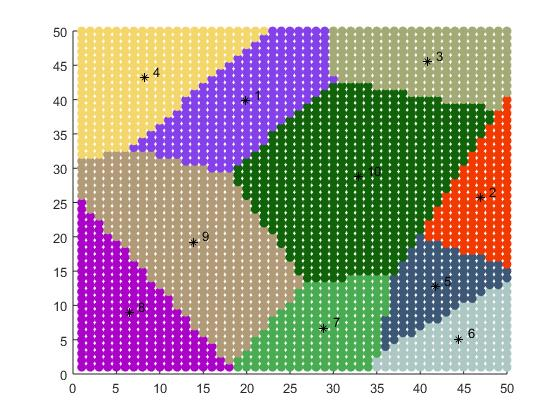
\includegraphics[width=0.8\linewidth]{figure/2omtcell2}
\caption{50*50 regular mesh with 10 data injection community division}
\label{2omtcell2}
\end{figure}

The speedup ratio as follows:
\\
The initial speedup figure. Fig.\ref{2voronoicurve}

\begin{figure}[h]
\centering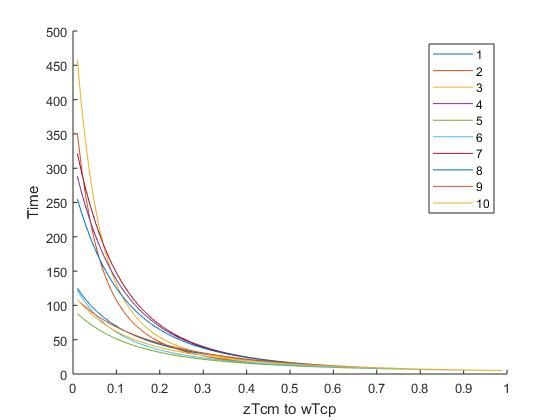
\includegraphics[width=0.8\linewidth]{figure/2voronoicurve}
\caption{Speedup vs $\sigma$ in different community division}
\label{2voronoicurve}
\end{figure}

Re-balance Voronoi optimization speedup figure Fig.\ref{2voronoicurve2}
\\
\begin{figure}[h]
\centering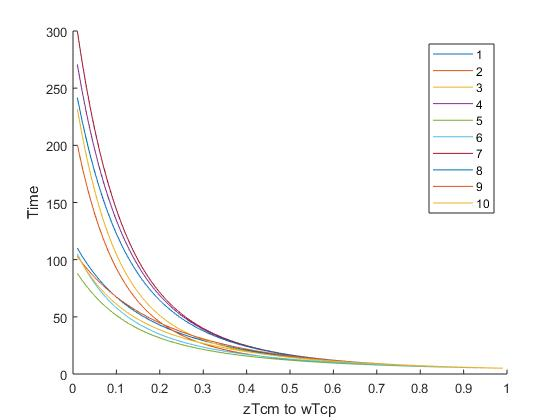
\includegraphics[width=0.8\linewidth]{figure/2voronoicurve2}
\caption{Speedup vs $\sigma$ in different community division}
\label{2voronoicurve2}
\end{figure}

The optimal mass transport speedup figure Fig.\ref{2voronoicurve3}
\\
\begin{figure}[h]
\centering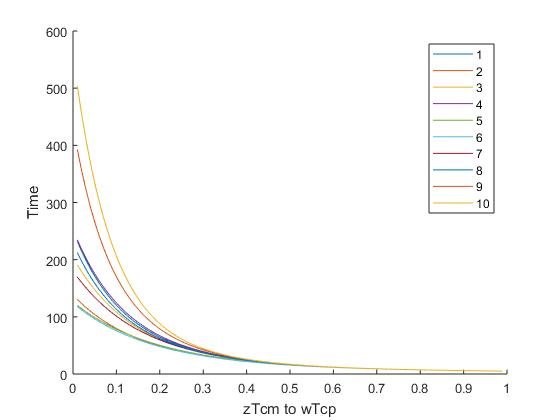
\includegraphics[width=0.8\linewidth]{figure/2voronoicurve3}
\caption{Speedup vs $\sigma$ in different community division}
\label{2voronoicurve3}
\end{figure}


\section{Experiment}



\section{Conclusion}


%% The Appendices part is started with the command \appendix;
%% appendix sections are then done as normal sections
%% \appendix

%% \section{}
%% \label{}

%% References
%%
%% Following citation commands can be used in the body text:
%% Usage of \cite is as follows:
%%   \cite{key}          ==>>  [#]
%%   \cite[chap. 2]{key} ==>>  [#, chap. 2]
%%   \citet{key}         ==>>  Author [#]

%% References with bibTeX database:

\bibliographystyle{model1-num-names}
\bibliography{sample.bib}

%% Authors are advised to submit their bibtex database files. They are
%% requested to list a bibtex style file in the manuscript if they do
%% not want to use model1-num-names.bst.

%% References without bibTeX database:

% \begin{thebibliography}{00}

%% \bibitem must have the following form:
%%   \bibitem{key}...
%%

% \bibitem{}

% \end{thebibliography}


\end{document}

%%
%% End of file `elsarticle-template-1-num.tex'.